\documentclass[aspectratio=169]{beamer}

\usepackage[T1]{fontenc}
\usepackage[utf8]{inputenc}
\usepackage[english]{babel}
\usepackage{pgfplots}
\pgfplotsset{compat=newest}
\usepackage{booktabs}
\usepackage{siunitx}

%\usepackage{natbib}
%\usepackage[style=apa, backend = bibtex]{biblatex}
\usepackage[numbers]{natbib}
\usepackage{bibentry}
\usepackage{graphicx} % Allows including images
\usepackage{booktabs} % Allows the use of \toprule,
%\usepackage{subcaption}
\usepackage{subfig}
% Latin Modern
\usepackage{lmodern}
\usepackage{multimedia}
%\usepackage{animate}
\usepackage{xmpmulti}
% Verdana font type
%\usepackage{verdana}
% Helvetica
%\usepackage{helvet}
% Times (text and math)
%\usepackage{newtx, newtxmath}

\usetheme[department=compute]{DTU}

\title[Applied 3D Vision]{Applied 3D Vision}
\author{Sebastian Hoppe Nesgaard Jensen}
\institute{Image Analysis \& Computer Graphics}
\date{\today}

\newcommand{\tabitem}{{\color{dtured}$\bullet$} }
%\setcounter{subsection}{1}
\useoutertheme{miniframes}
\AtBeginSection[]{\subsection{}}

\begin{document}
\nobibliography*
\frame{
	\maketitle
}

\section{Introduction}

\frame{
  \frametitle{Part of}
  \begin{figure}
    
\includegraphics[width=0.8\textwidth]{figures/madelogo}
  \end{figure}
  Workpackage 8: Hyperflexible Automation
}
\frame{
  \frametitle{3D Vision}
  \begin{minipage}[t]{0.48\linewidth}
    \begin{itemize}
      \item Use readily available 3D sensors.
      \item Solve problems.
      \item Both industrial and academic.
    \end{itemize}
  \end{minipage}
  \begin{minipage}[t]{0.48\linewidth}
    \begin{figure}
      \includegraphics[width=1.0\linewidth]{figures/nrsfm_scanner}
    \end{figure}
  \end{minipage}
}

\begin{comment}
\frame{
  \frametitle{Commercial 3D Sensors}
  \begin{figure}
    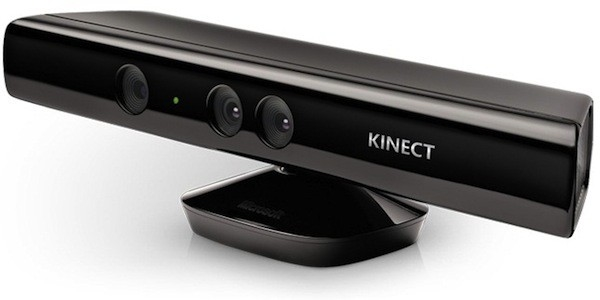
\includegraphics[width=0.35\linewidth]{figures/kinect}
    \hspace{2cm}
    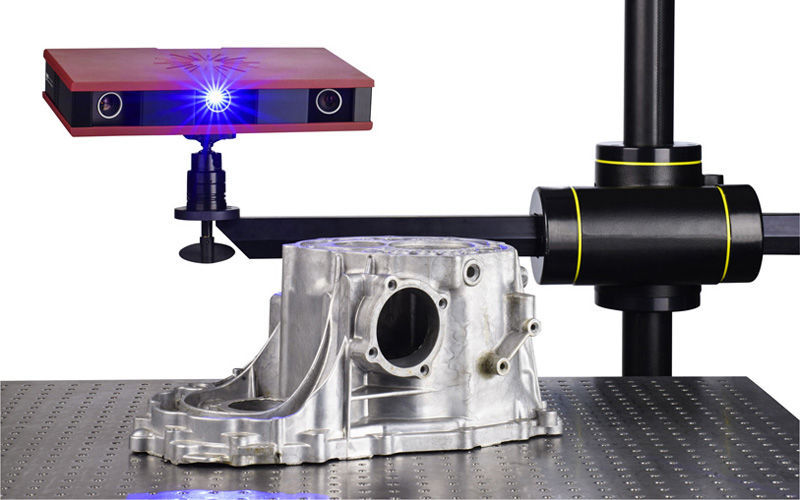
\includegraphics[width=0.35\linewidth]{figures/gom}
  \end{figure}
  \begin{figure}
    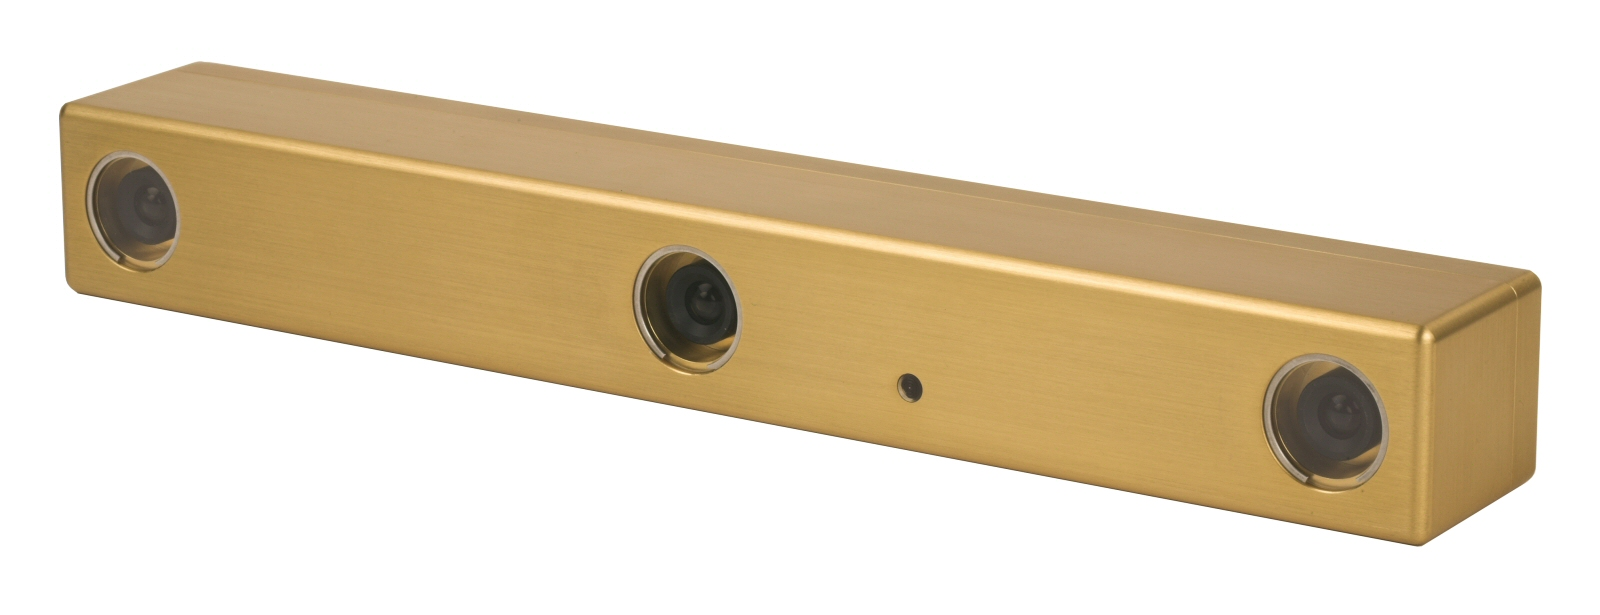
\includegraphics[width=0.35\linewidth]{figures/bumblebee}
    \hspace{2cm}
    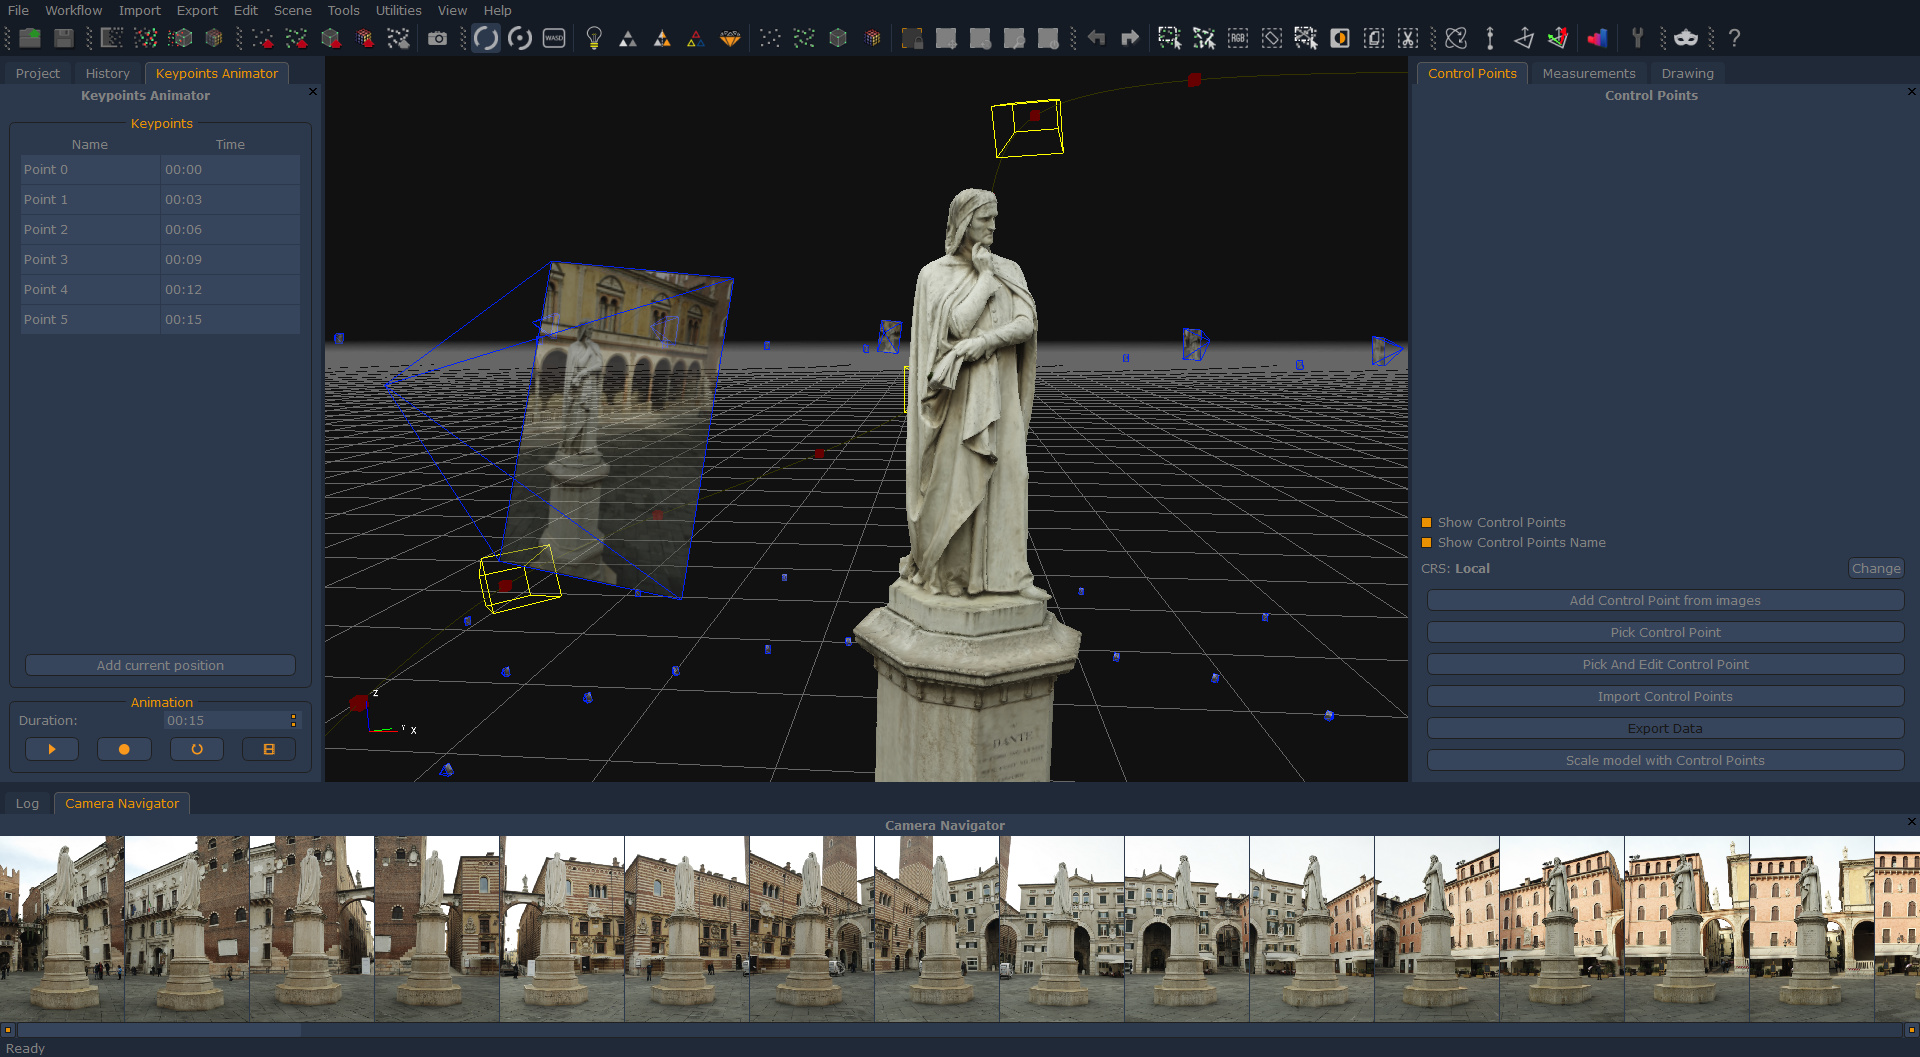
\includegraphics[width=0.35\linewidth]{figures/3df_zephyr_3_photogrammetry_statue}
  \end{figure}
}

\frame{
  \frametitle{3D Vision Application}
  \begin{figure}[t]
    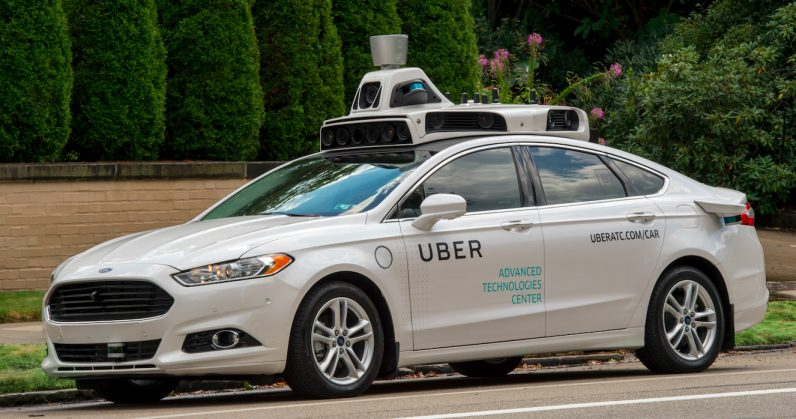
\includegraphics[width=0.47\linewidth]{figures/selfdriving}
    \hfill
    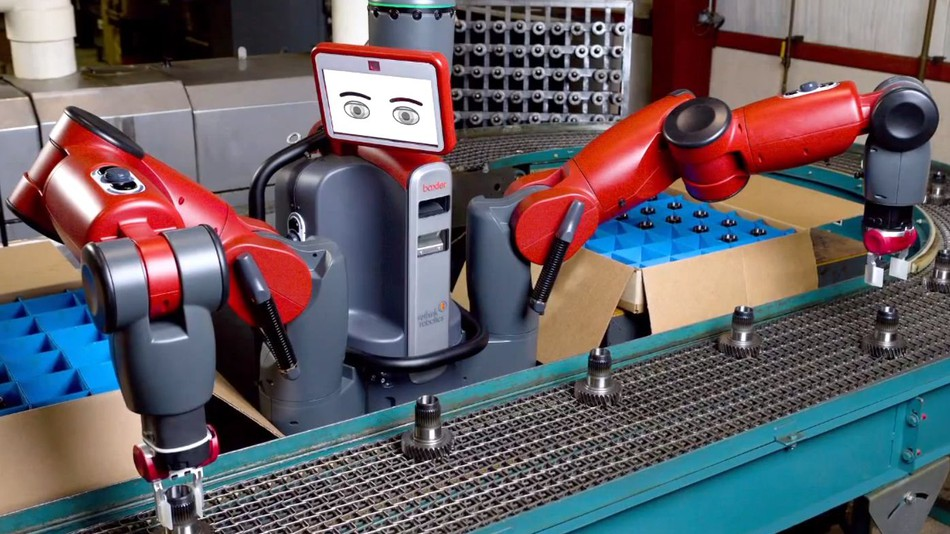
\includegraphics[width=0.47\linewidth]{figures/baxter}
  \end{figure}
}

\frame{
  \frametitle{Real-world application can be surprisingly tricky...}
  \begin{figure}
    \centering
    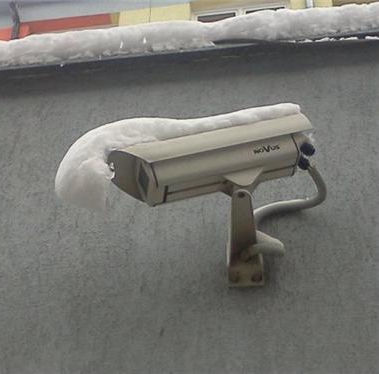
\includegraphics[height=0.65\textheight]{figures/icecam}
    \hfill
    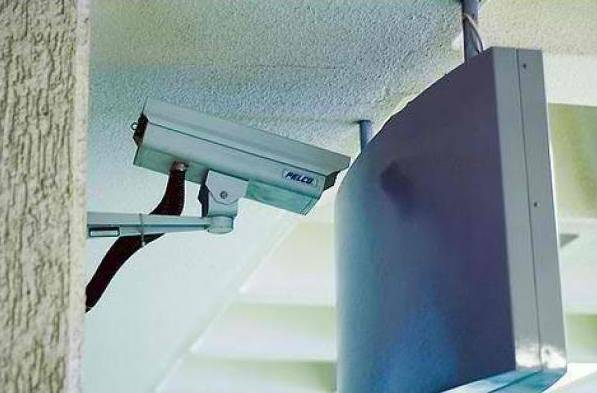
\includegraphics[height=0.65\textheight]{figures/failed2}
  \end{figure}
}
\end{comment}

\frame{
  \frametitle{Todays Topics}
  \tableofcontents
}

\section{Error Analysis of Structured Light}
\frame{
  \frametitle{An Error Analysis of Structured Light Scanning of Biological Tissue}
  Sebastian Nesgaard Jensen, Jakob Wilm, Henrin Aanæs

  \textit{SCIA 2017}
  \begin{figure}
    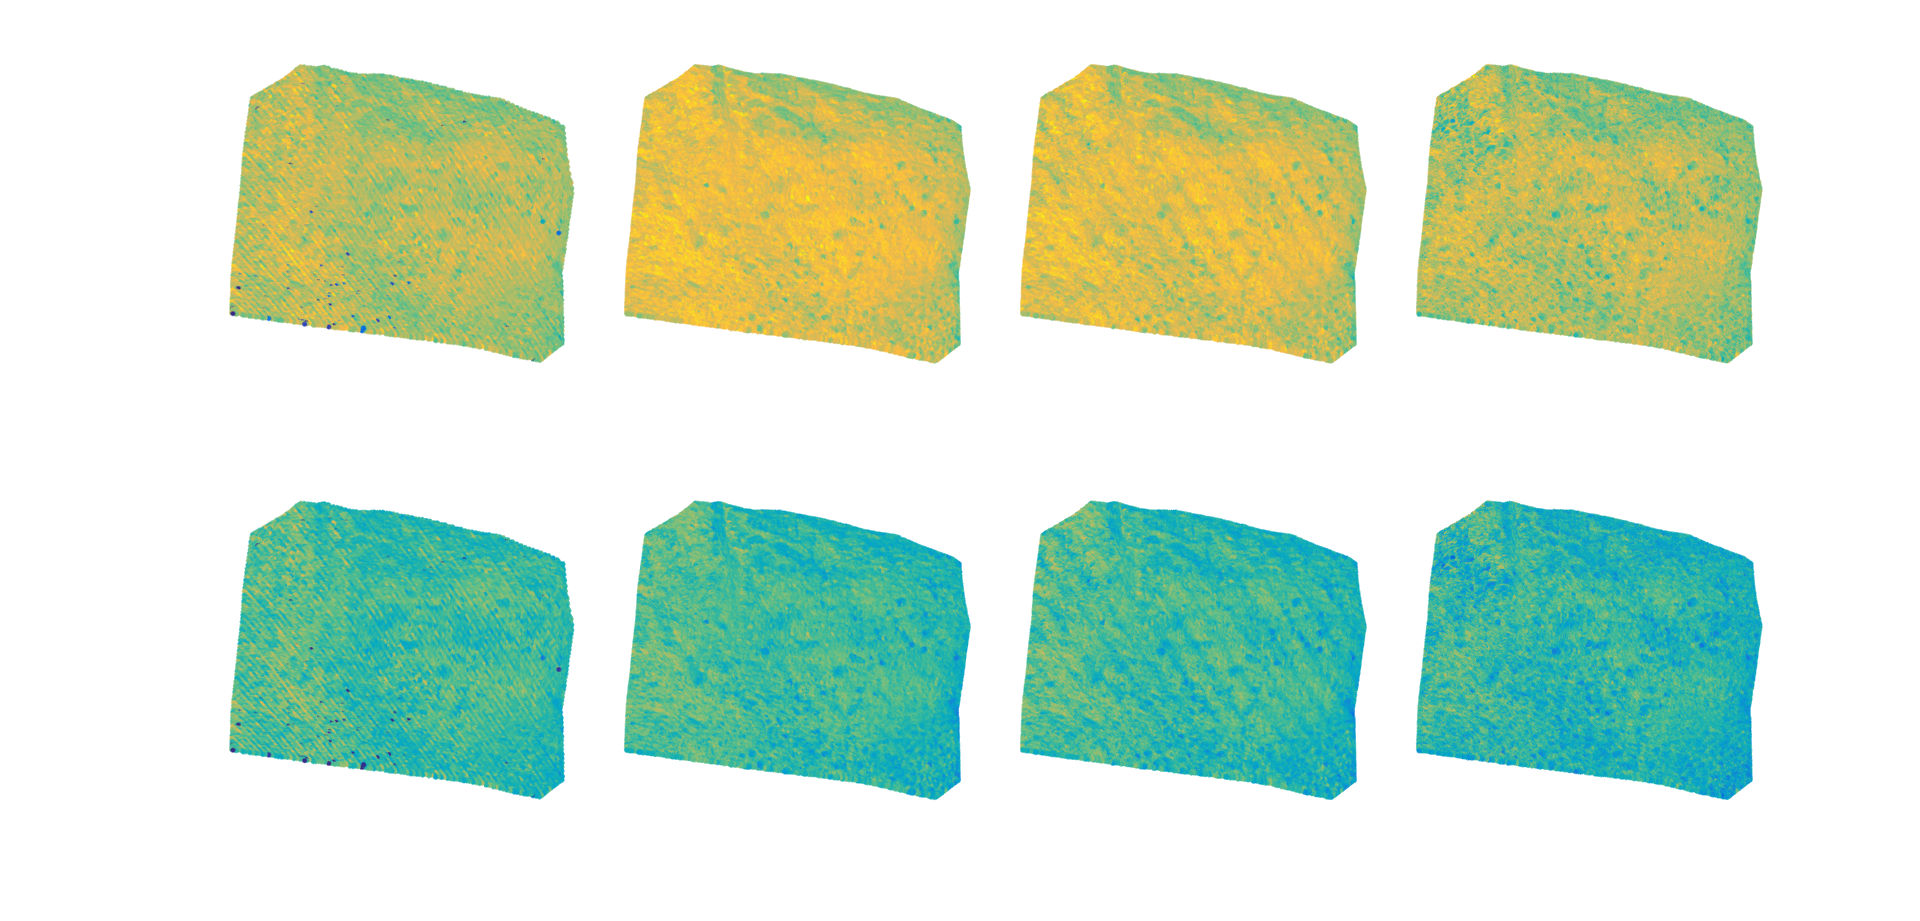
\includegraphics[width=0.80\linewidth]{figures/stlmeat}
      \hfill
  \end{figure}
  %\bibentry{jensen2017error}
}

\frame{
  \frametitle{Camera-Projector Structured Light}
  \begin{figure}
    \centering
    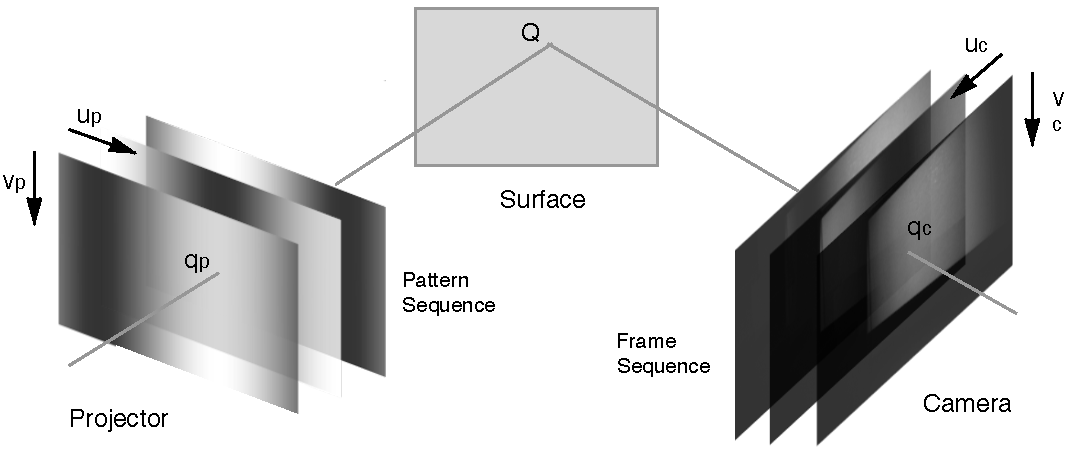
\includegraphics[width=0.80\linewidth]{figures/stl_principle}
  \end{figure}
}

\frame{
  \frametitle{Basic Ray Model}
  \begin{onlyenv}<1>
    \begin{figure}
      \centering
      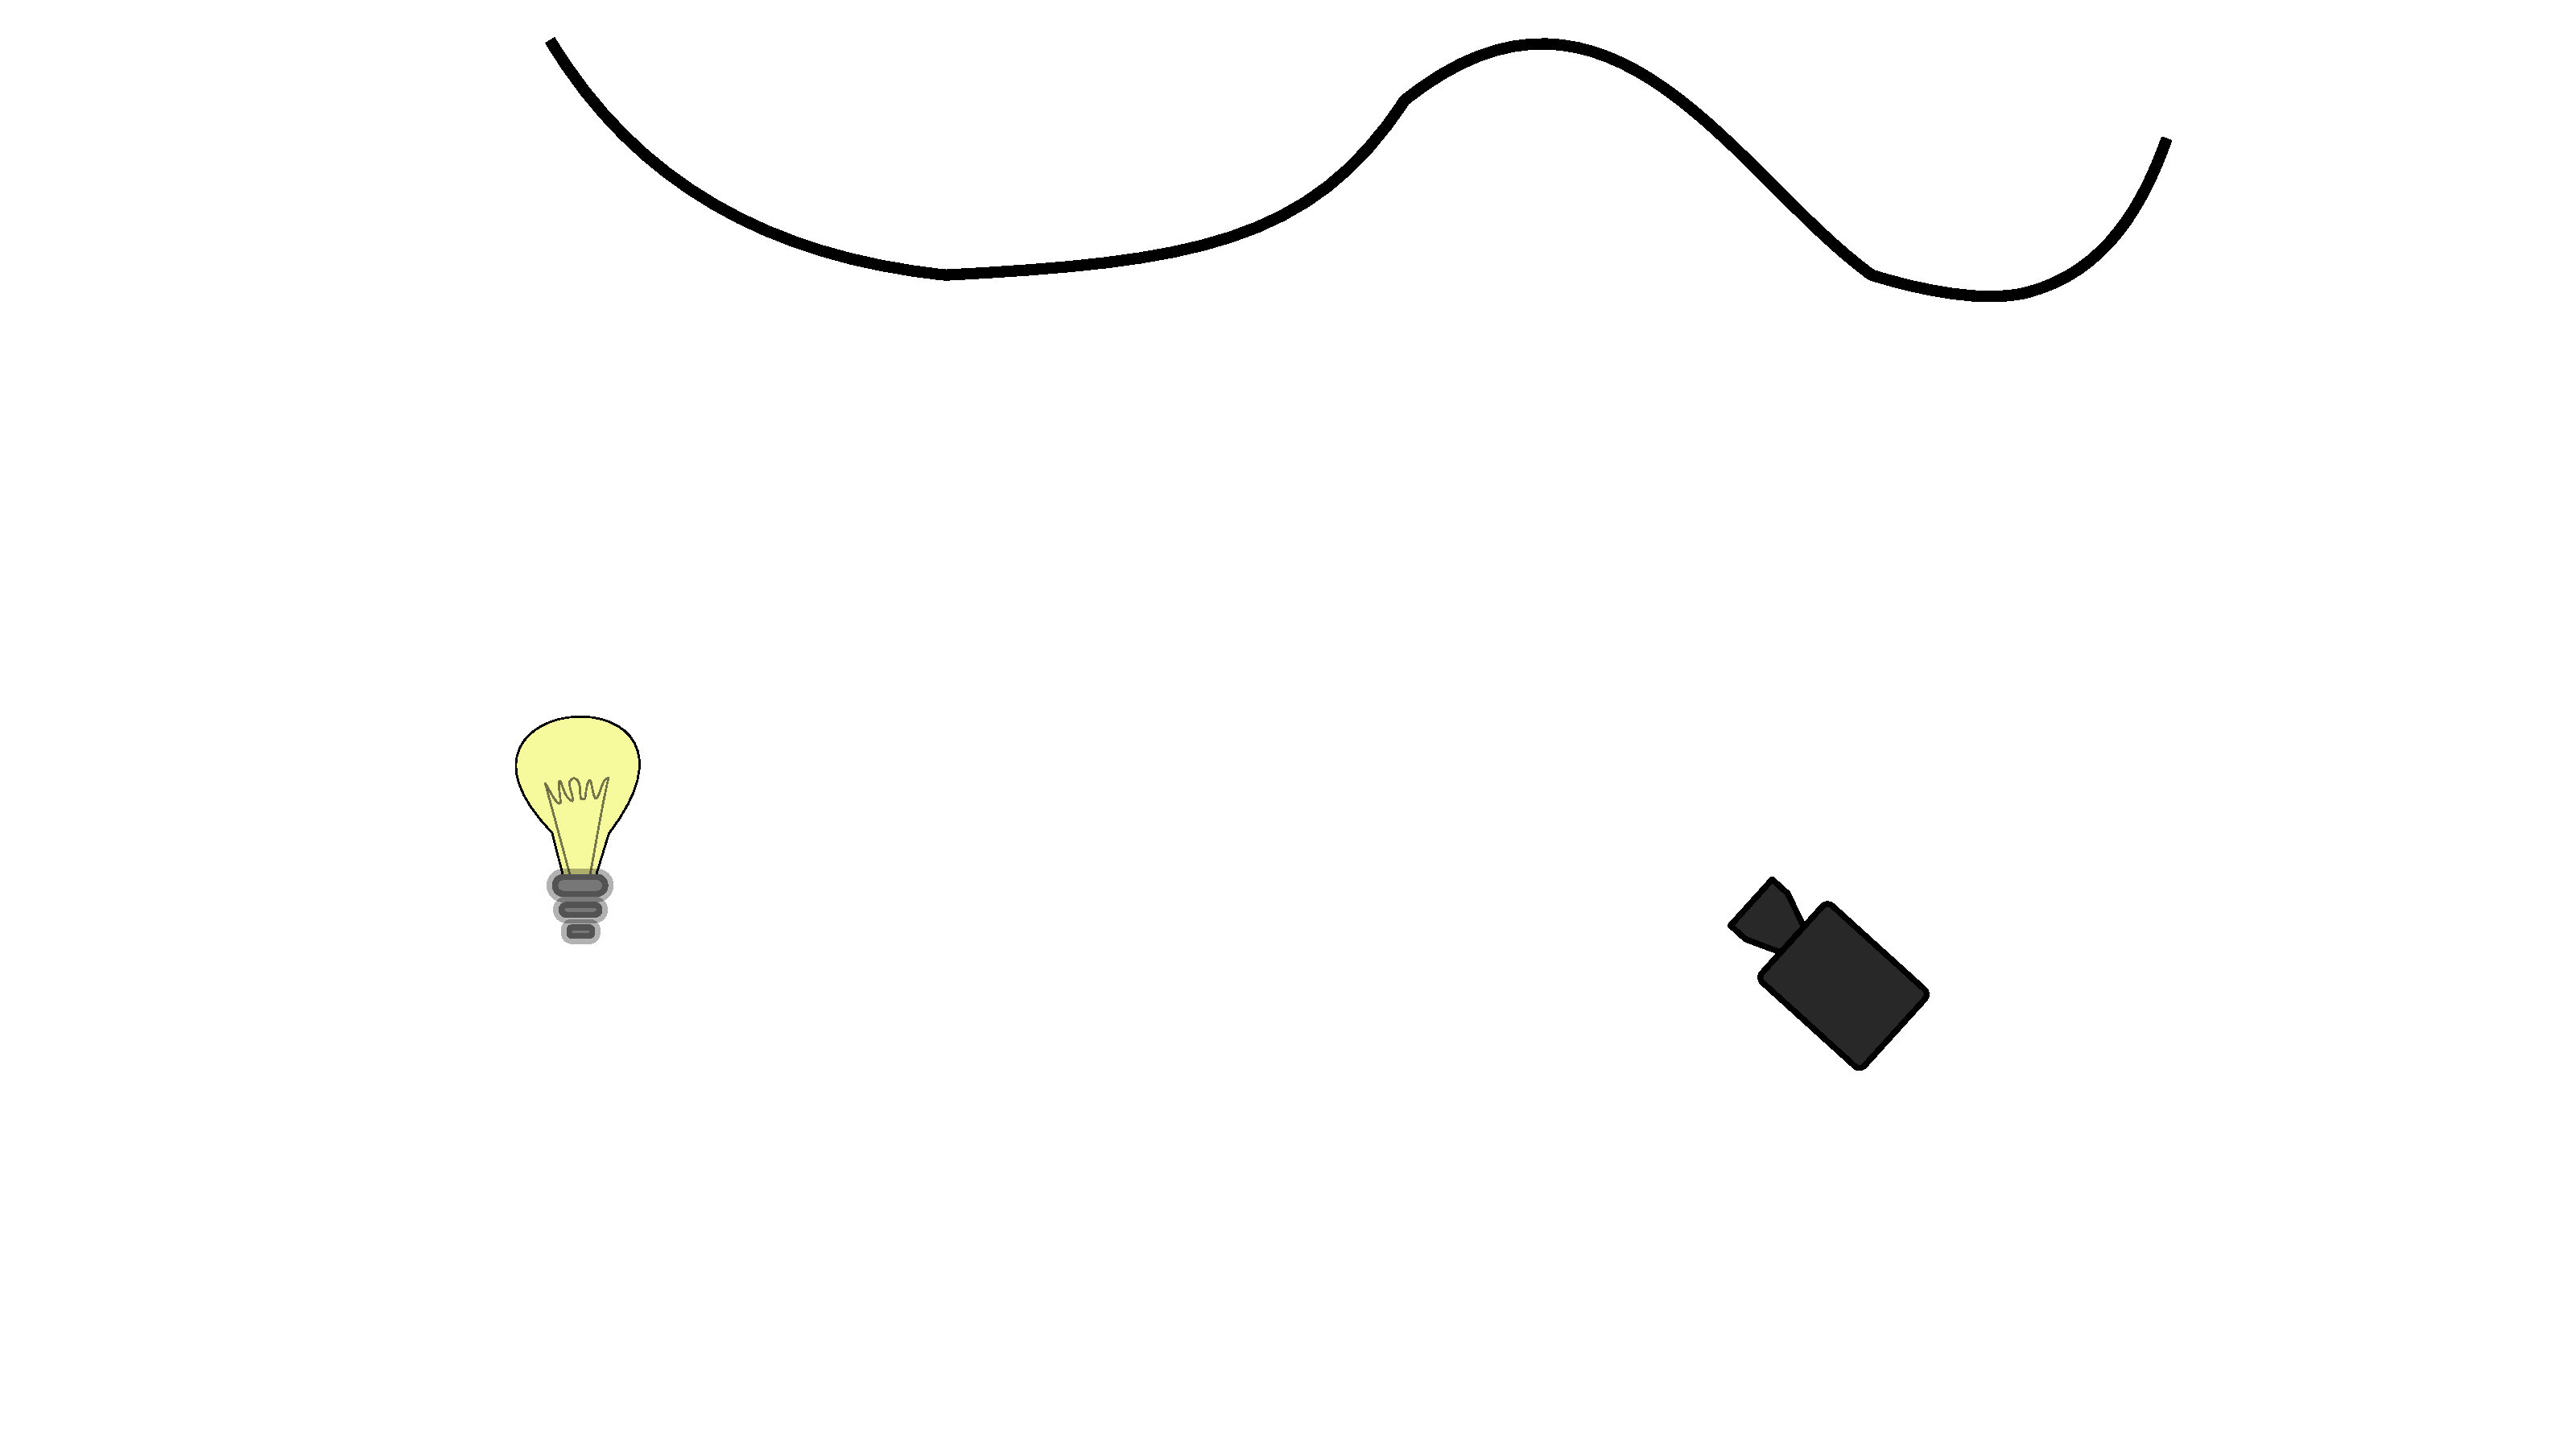
\includegraphics[width=0.8\linewidth]{figures/stl_none}
    \end{figure}
  \end{onlyenv}
  \begin{onlyenv}<2>
    \begin{figure}
      \centering
      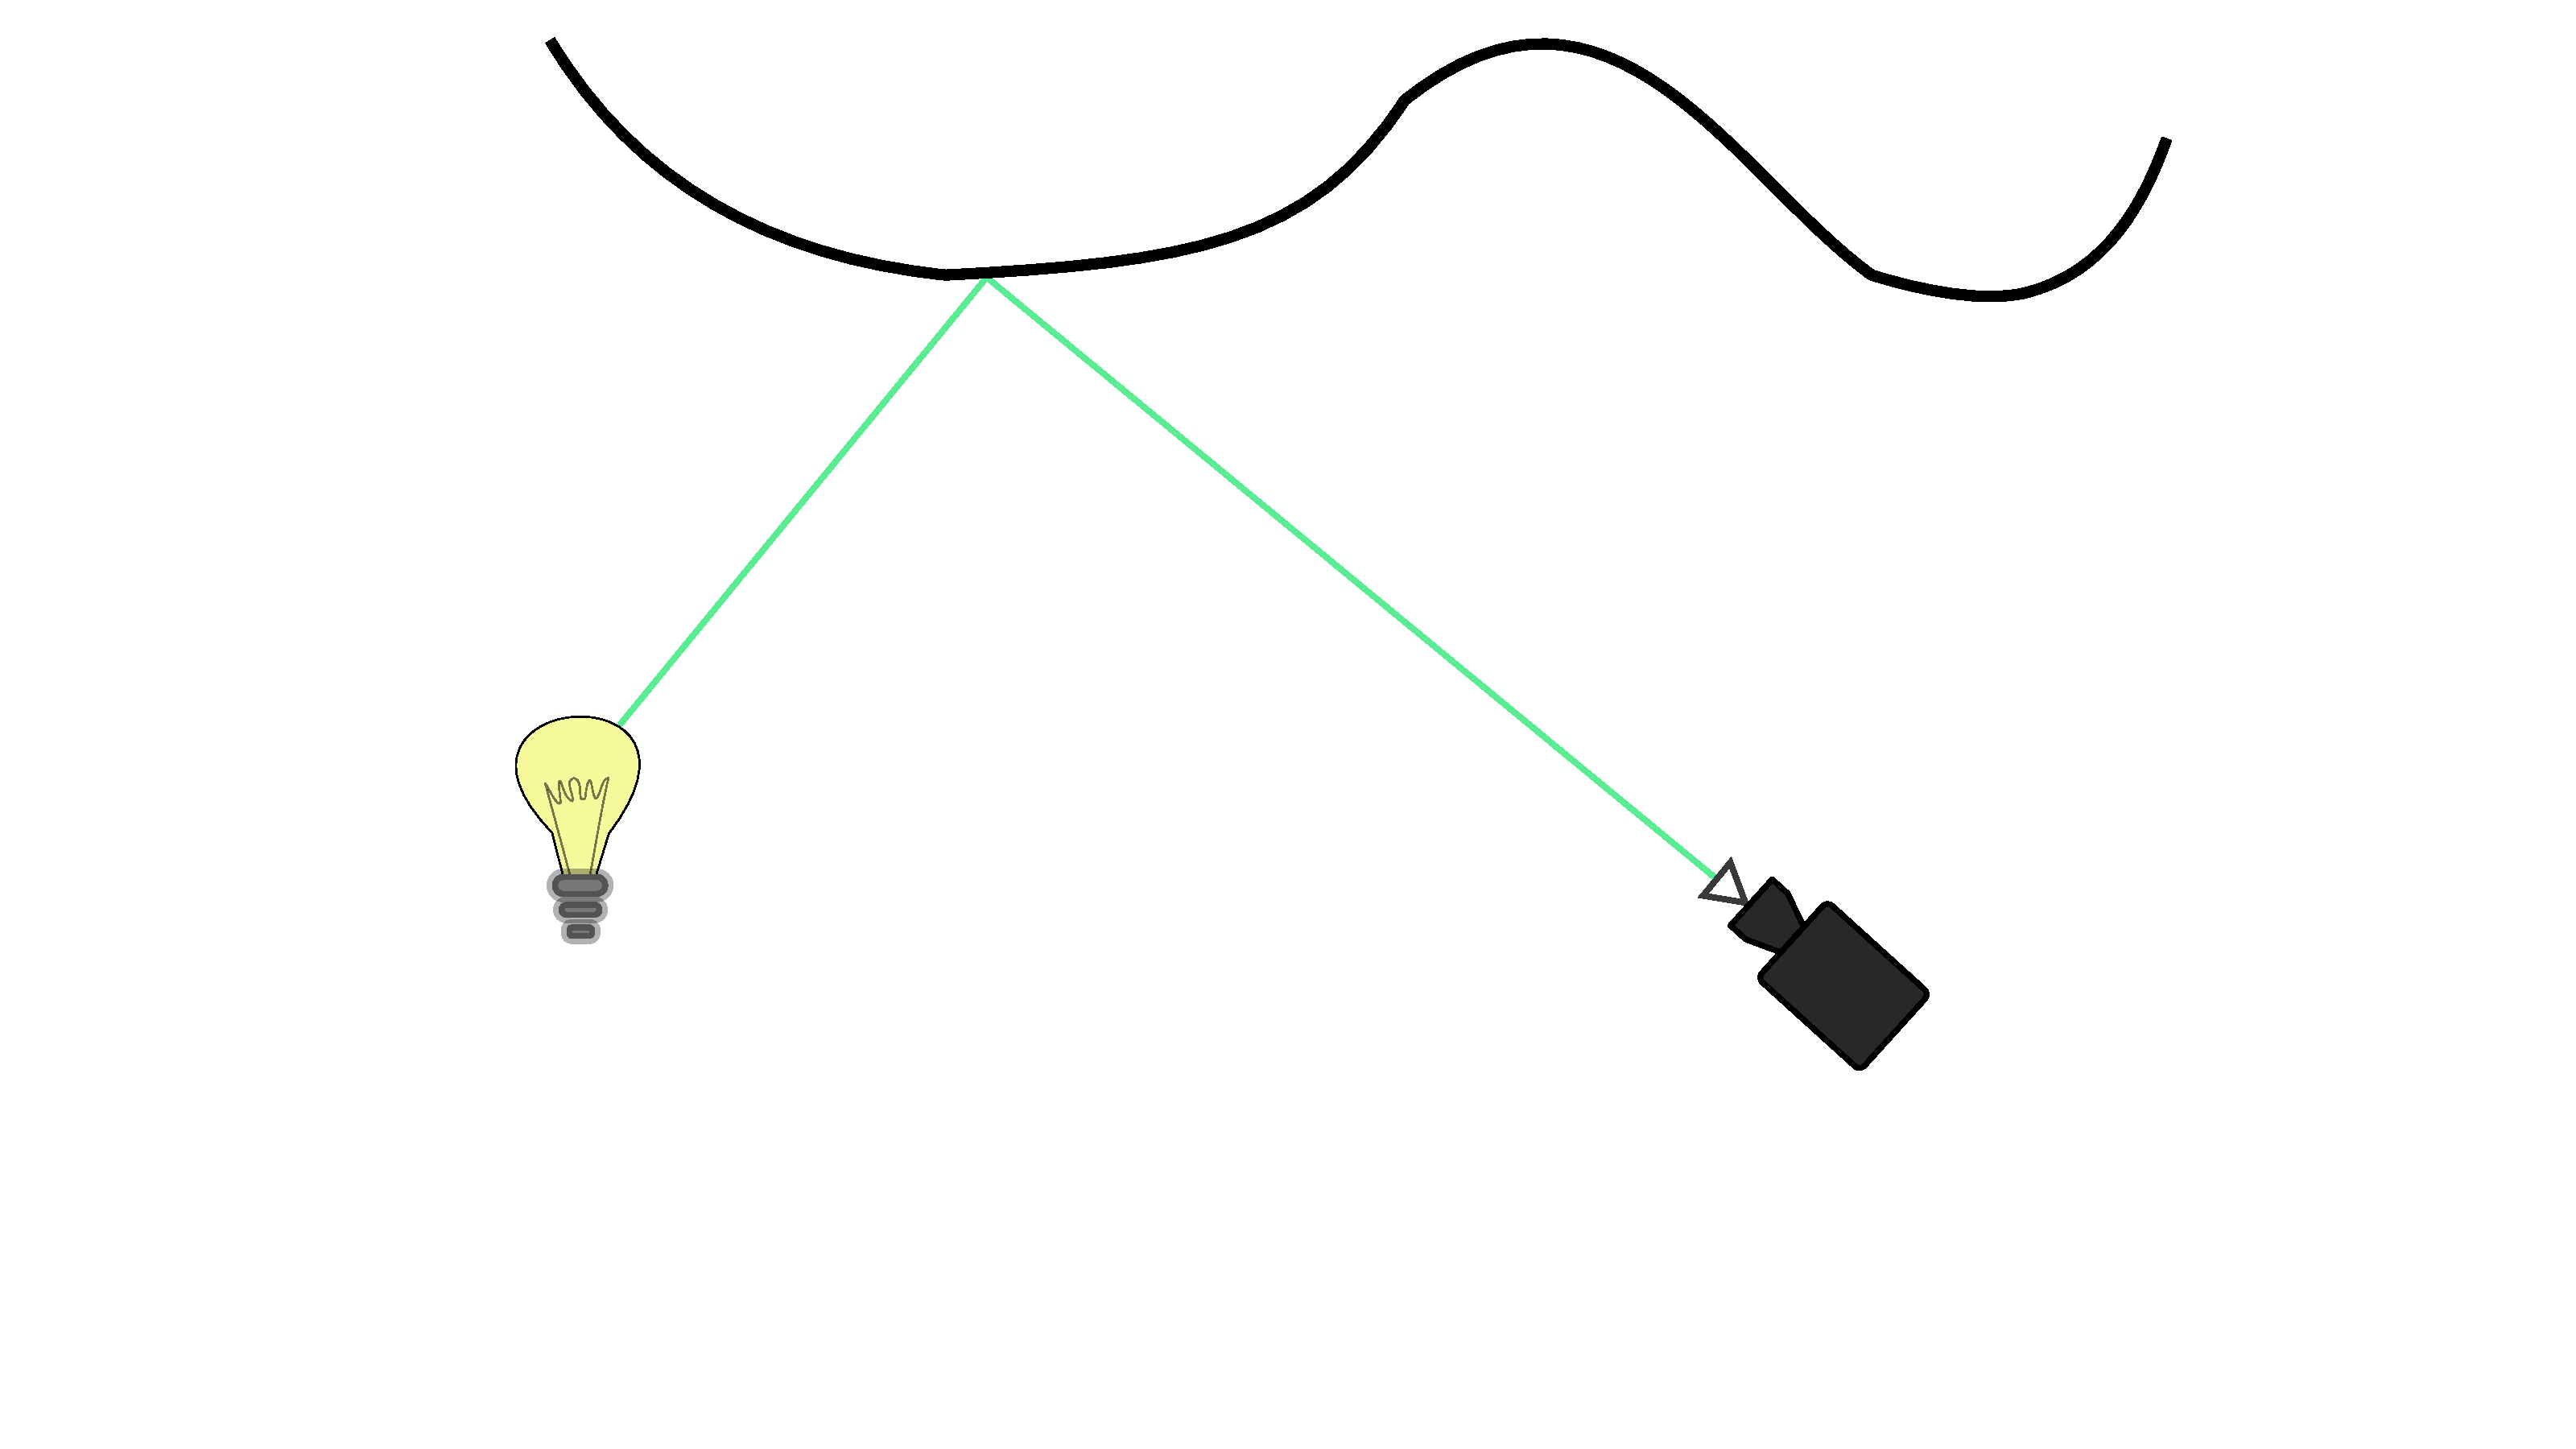
\includegraphics[width=0.8\linewidth]{figures/stl_direct}
    \end{figure}
  \end{onlyenv}
  \begin{onlyenv}<3>
    \begin{figure}
      \centering
      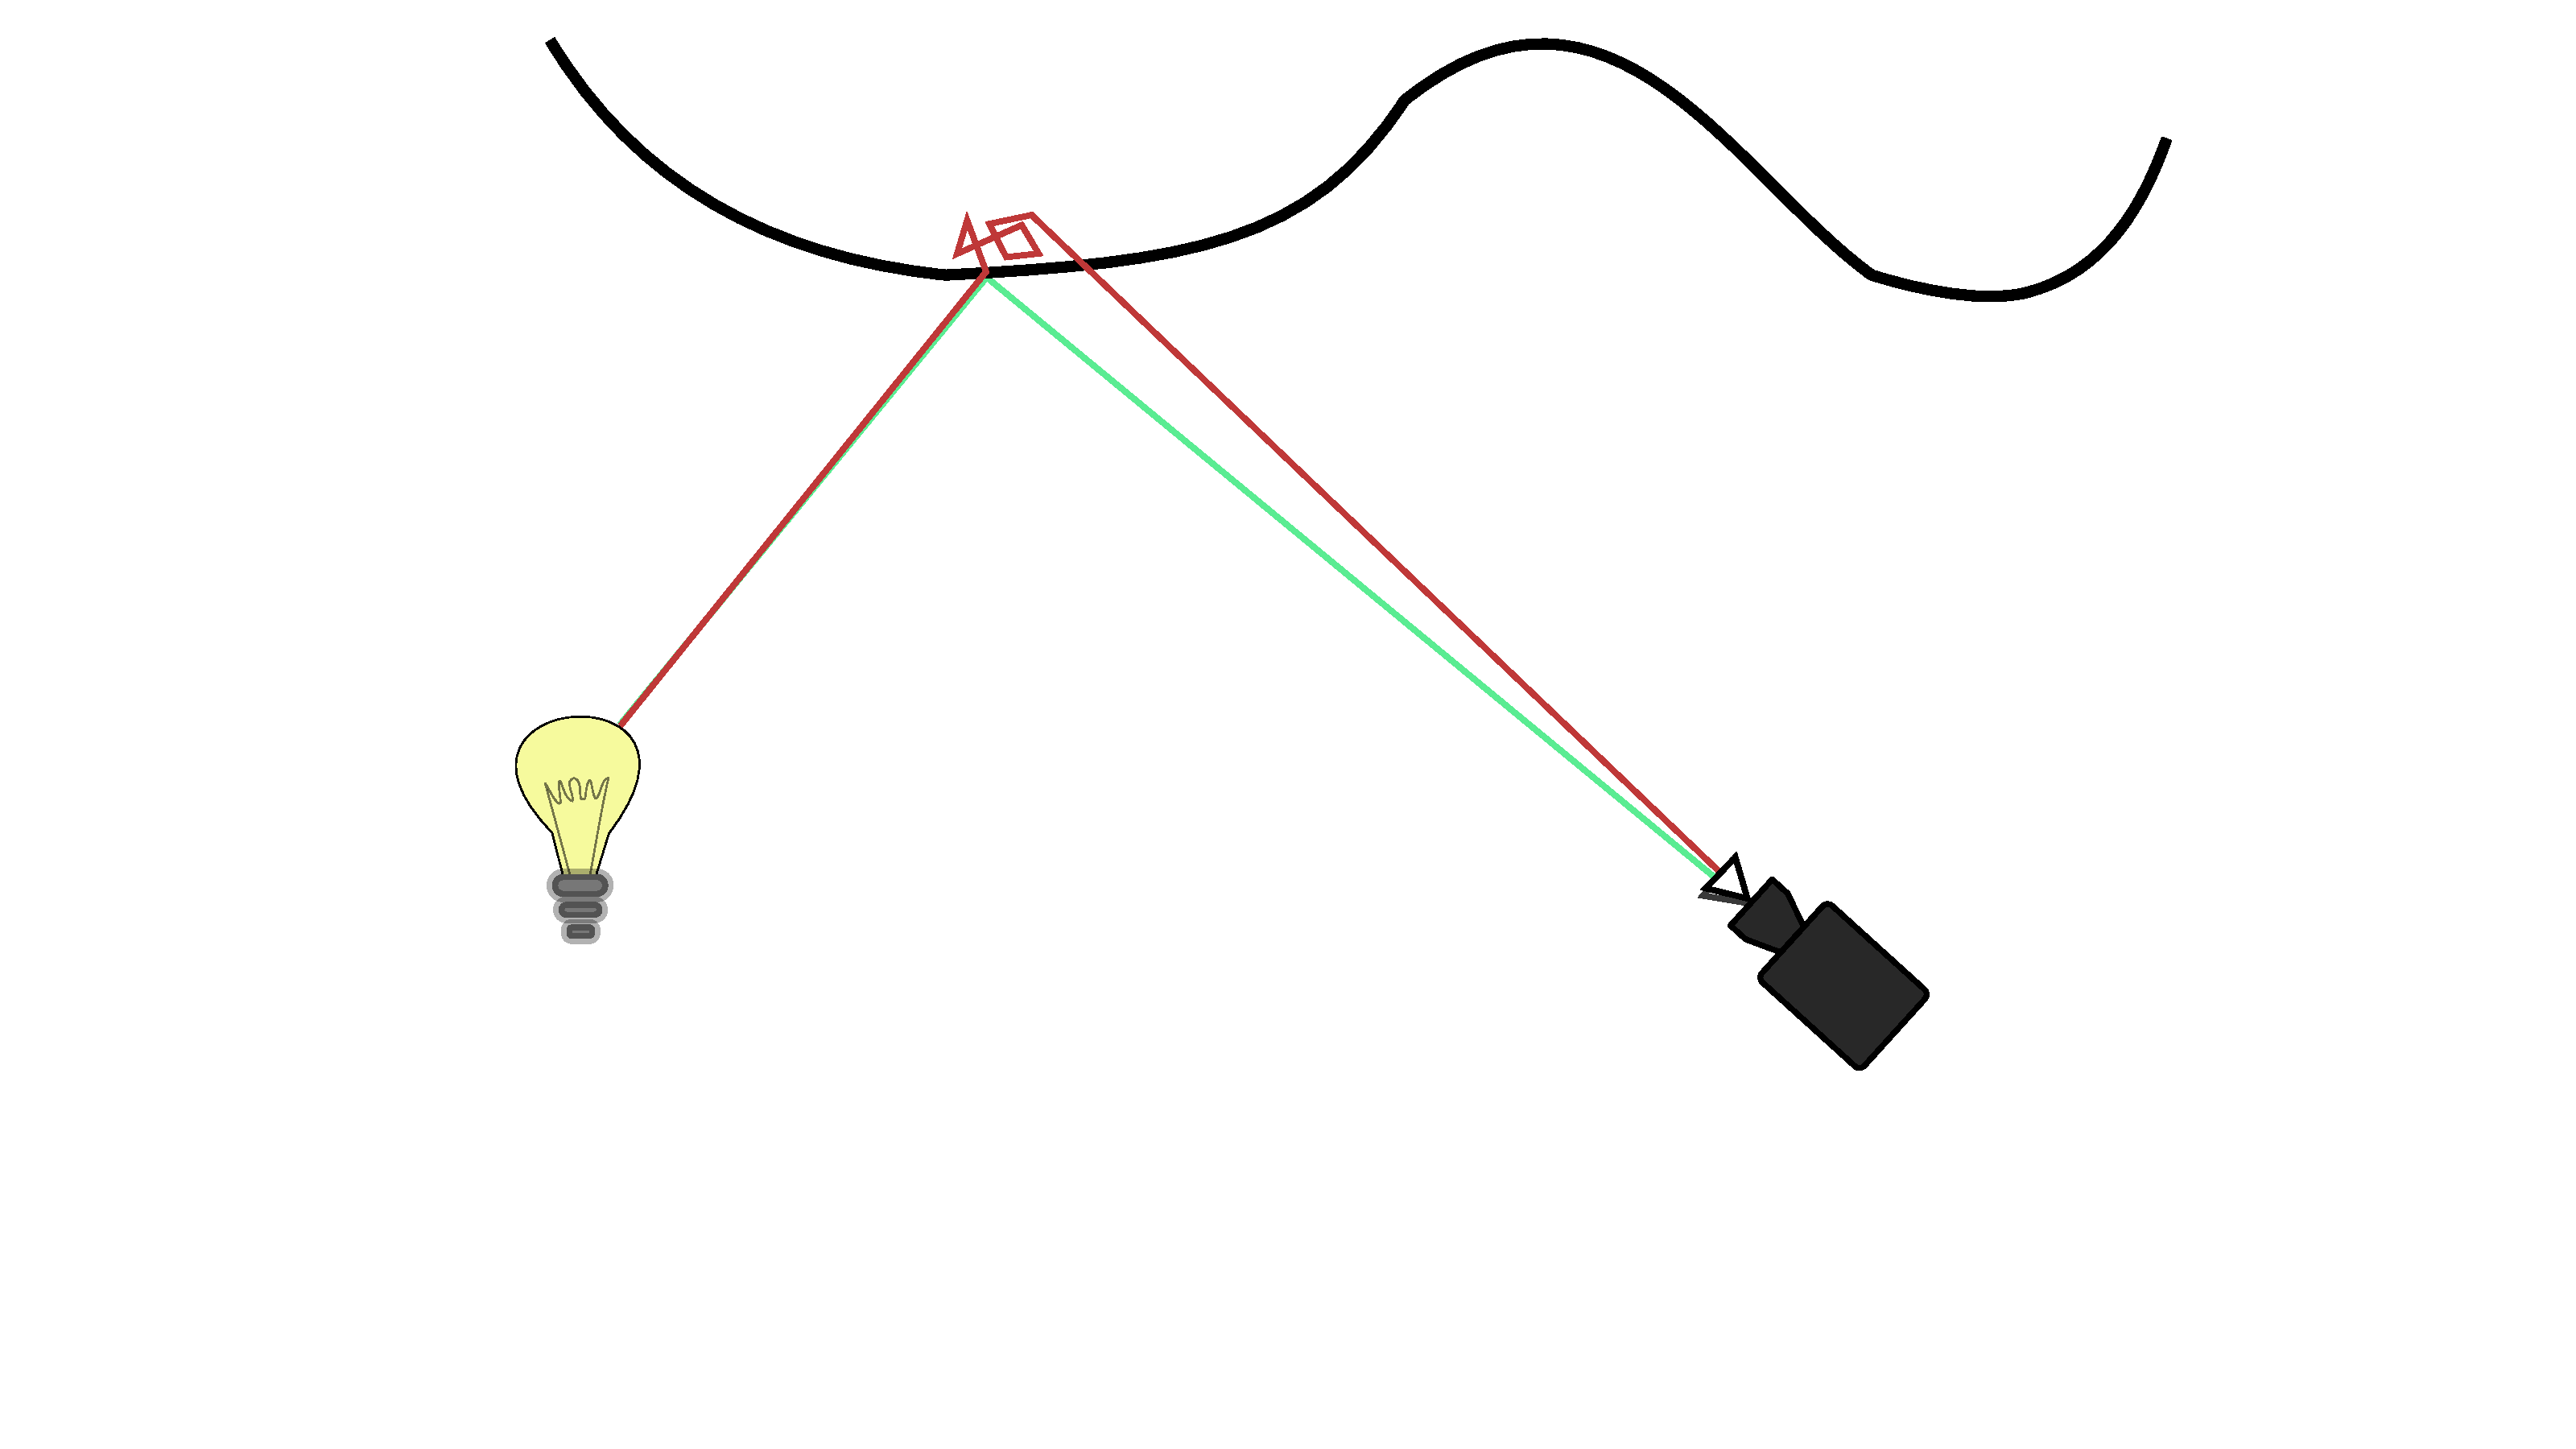
\includegraphics[width=0.8\linewidth]{figures/stl_all}
    \end{figure}
  \end{onlyenv}
}


\frame{
  \frametitle{Significance of Subsurface Scattering}
  \begin{figure}
    \centering
    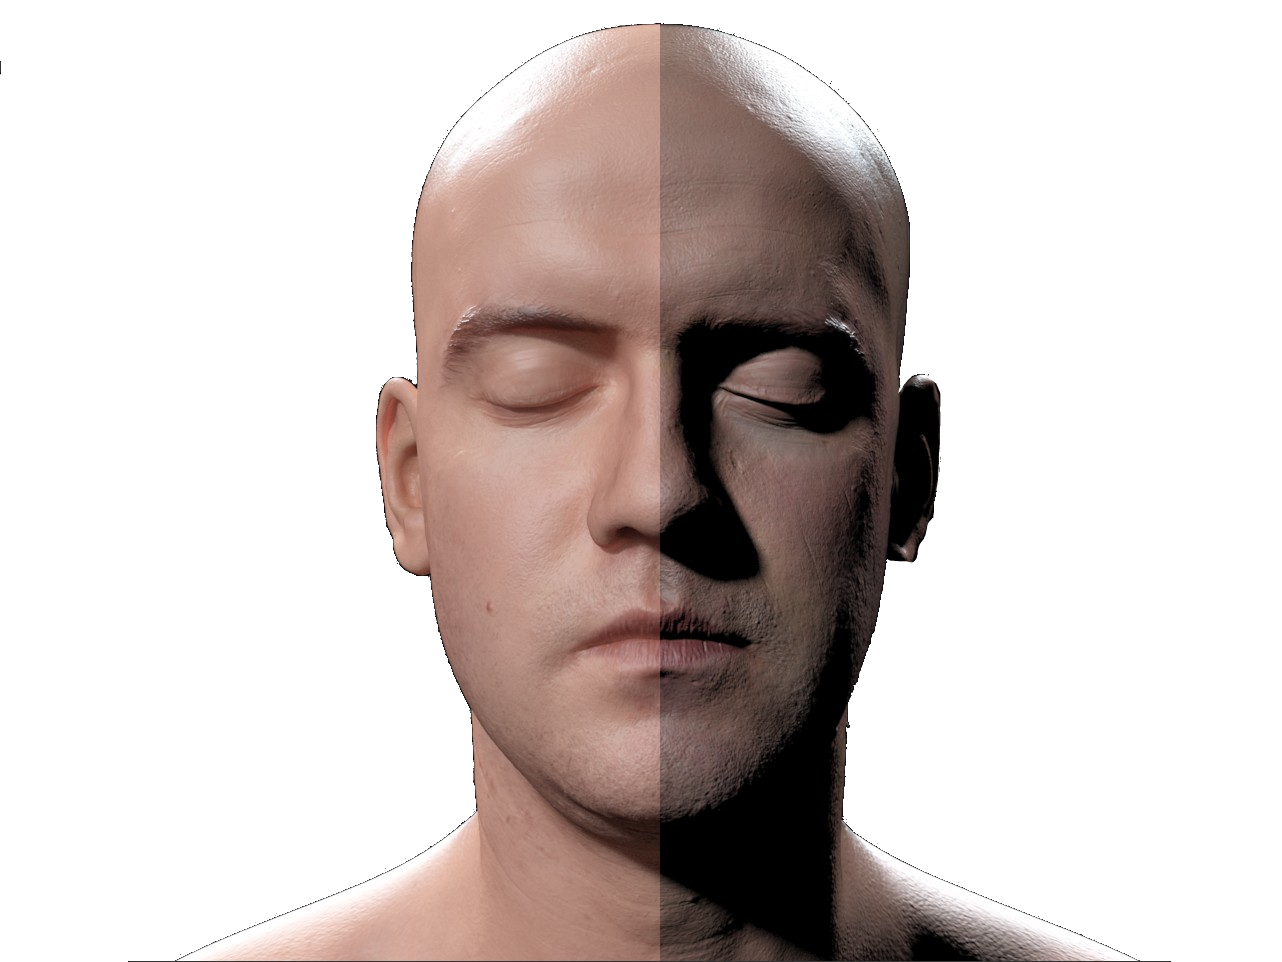
\includegraphics[height=0.8\textheight]{figures/humanss}
  \end{figure}
}

\frame{
  \frametitle{Materials and Structured Light Methods}
  \begin{minipage}[t]{0.48\linewidth}
    \captionsetup[subfloat]{position=above, labelformat=empty}
    \begin{figure}
      \subfloat[Skin]{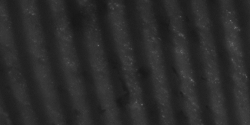
\includegraphics[width=0.49\linewidth]{figures/stlskinraw}}\hfill
      \subfloat[Fat]{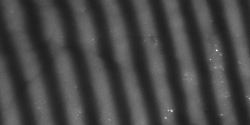
\includegraphics[width=0.49\linewidth]{figures/stlfatraw}}
    \end{figure}
    \captionsetup[subfloat]{position=below, labelformat=empty}
    \vspace{-1cm}
    \begin{figure}
      \subfloat[Meat]{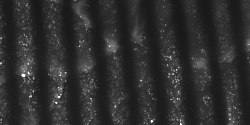
\includegraphics[width=0.49\linewidth]{figures/stlmuscleraw}}
    \end{figure}
  \end{minipage}\hfill
  \begin{minipage}[t]{0.48\linewidth}
    \captionsetup[subfloat]{position=above, labelformat=empty}
    \begin{figure}
      \subfloat[Gray Codes~\cite{posdamer1982surface}]{
\includegraphics[width=0.49\linewidth]{figures/pattern}}\hfill
      \subfloat[Phase Shifting~\cite{Huntley1993a}]{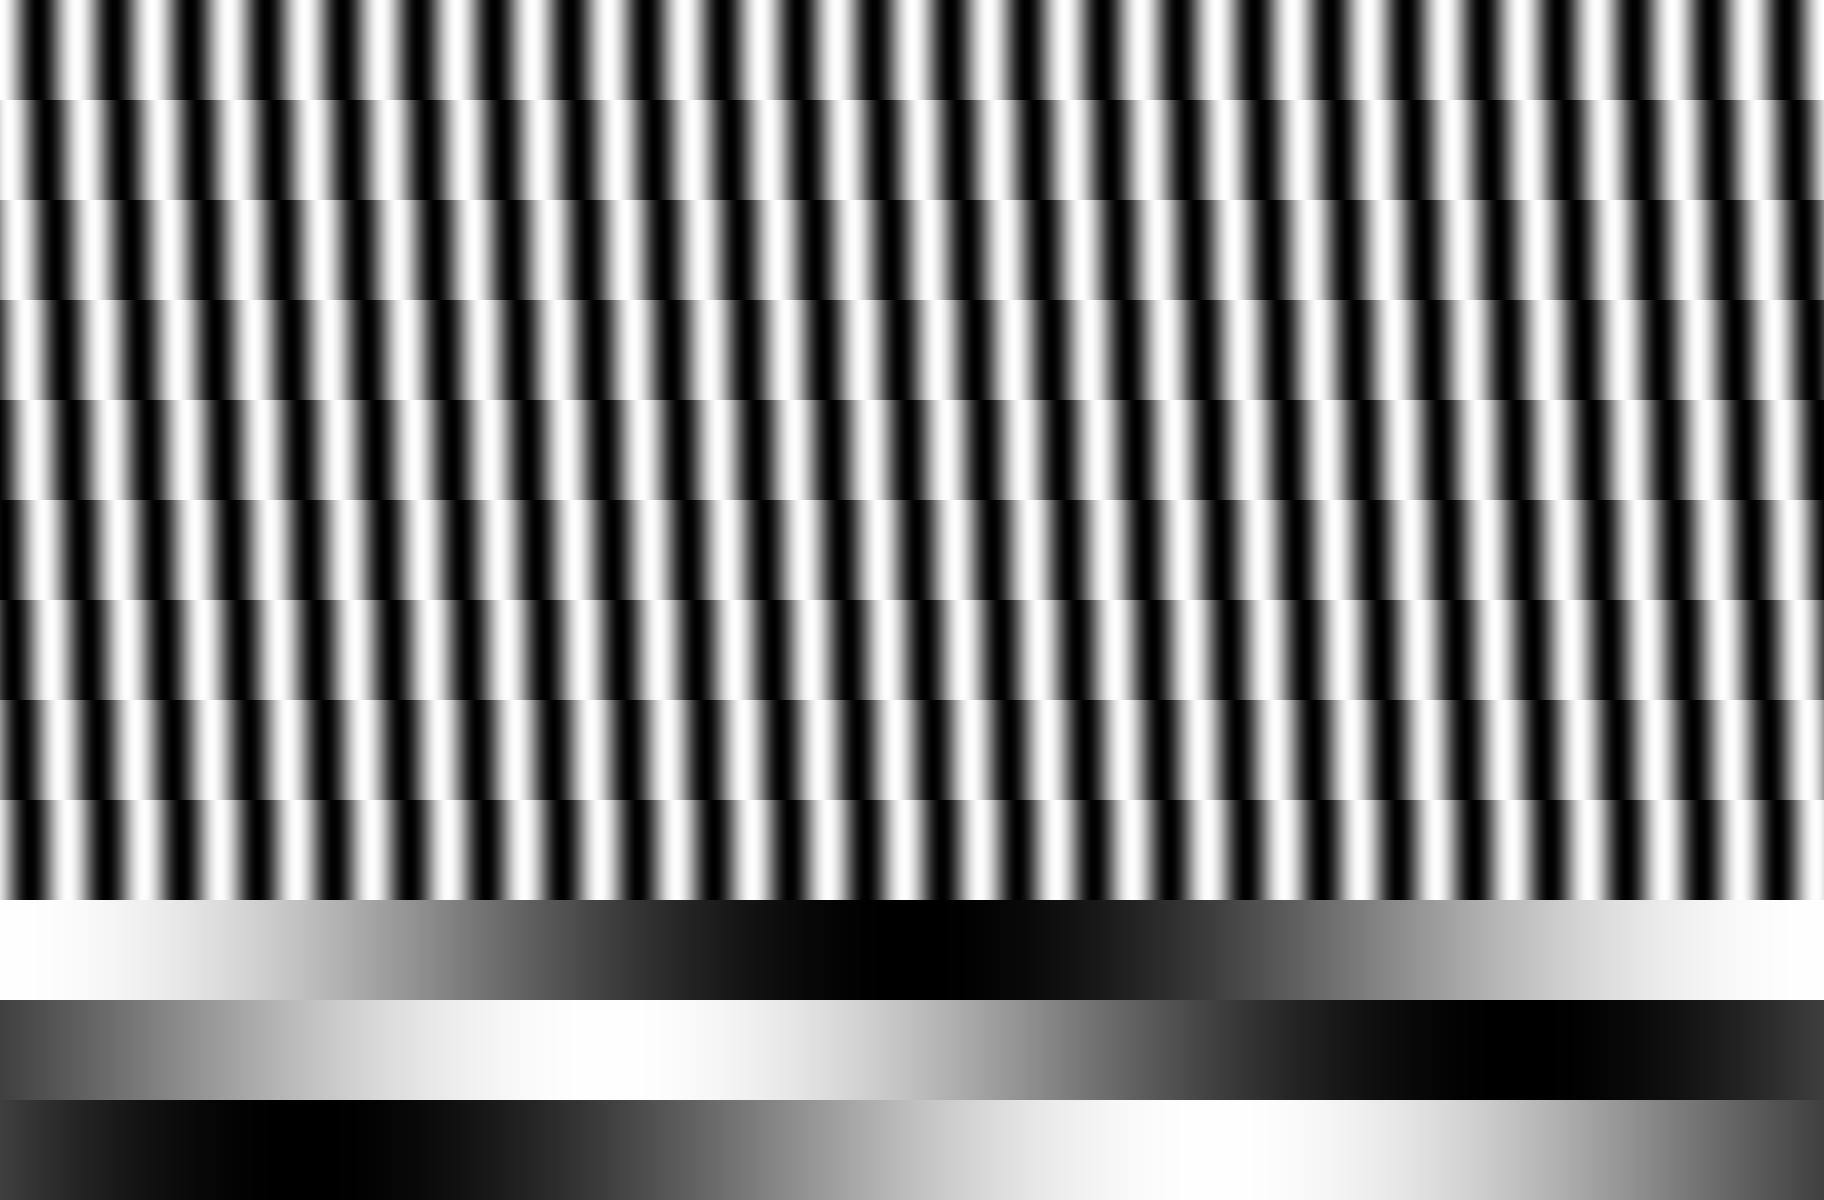
\includegraphics[width=0.49\linewidth]{figures/patterns_nstep}}
    \end{figure}
    \captionsetup[subfloat]{position=below, labelformat=empty}
    \vspace{-1cm}
    \begin{figure}
      \subfloat[Modulated Phase Shifting~\cite{chen2008modulated}]{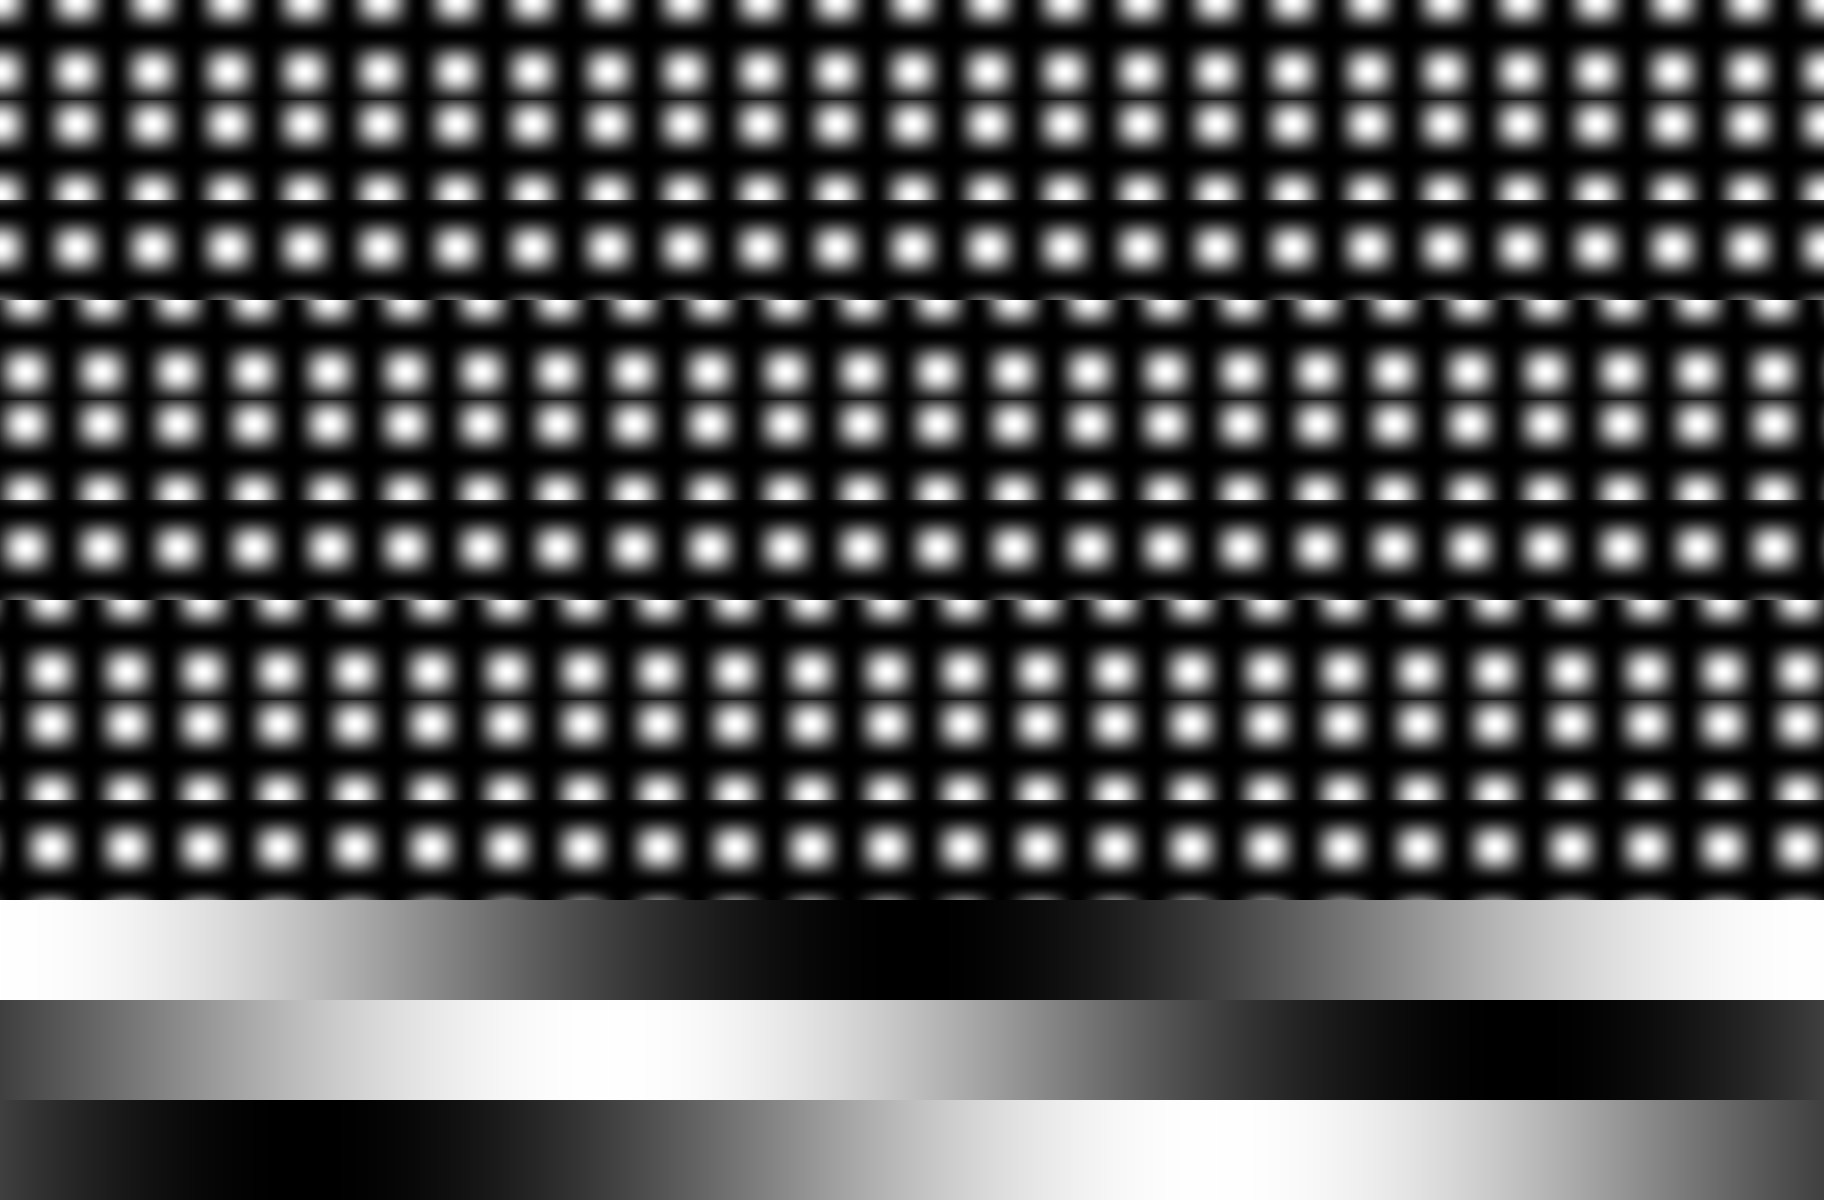
\includegraphics[width=0.49\linewidth]{figures/patterns_modulated}}\hfill
      \subfloat[Micro Phase Shifting~\cite{gupta2012micro}]{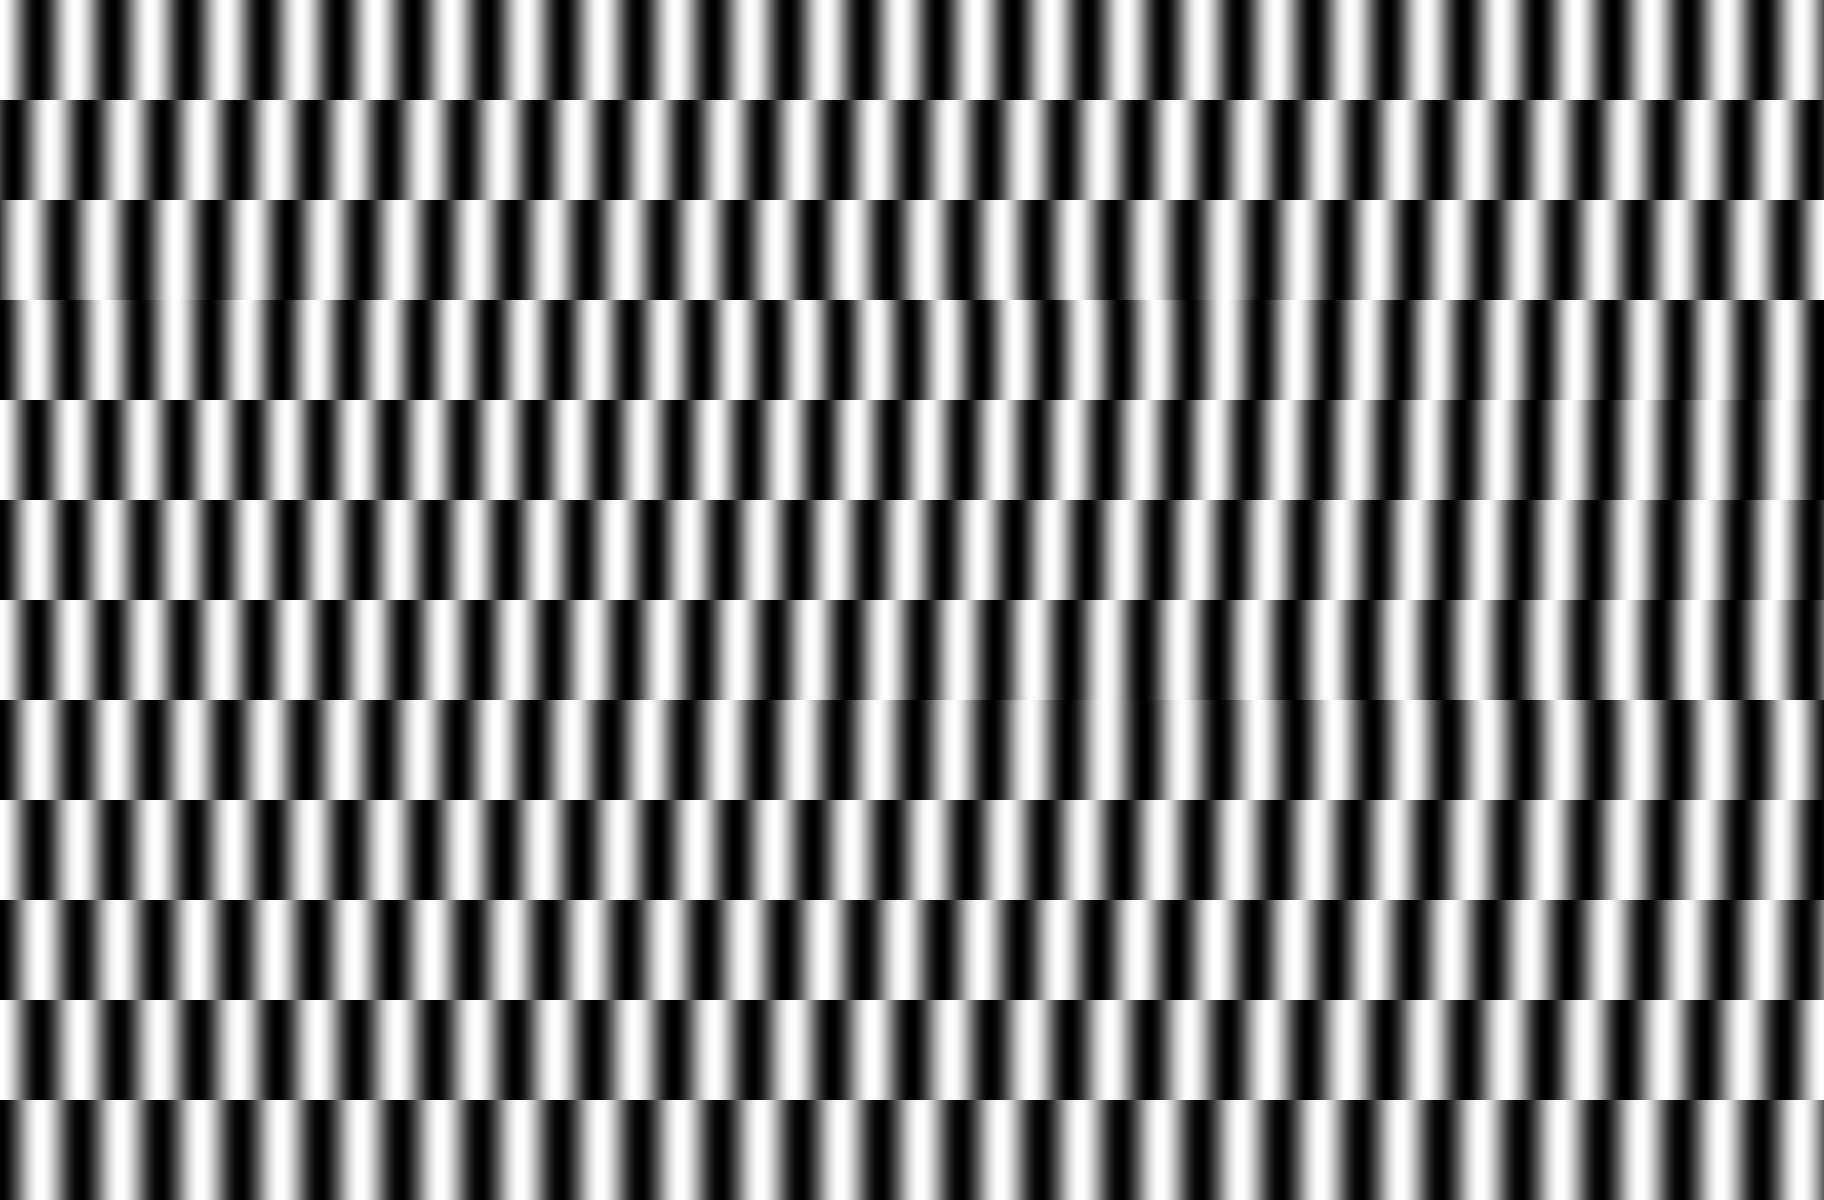
\includegraphics[width=0.49\linewidth]{figures/patterns_micro}}
    \end{figure}
  \end{minipage}
}

\frame{
  \frametitle{Reference Acquisition using Chalk Coating}
  \begin{figure}
    \centering
    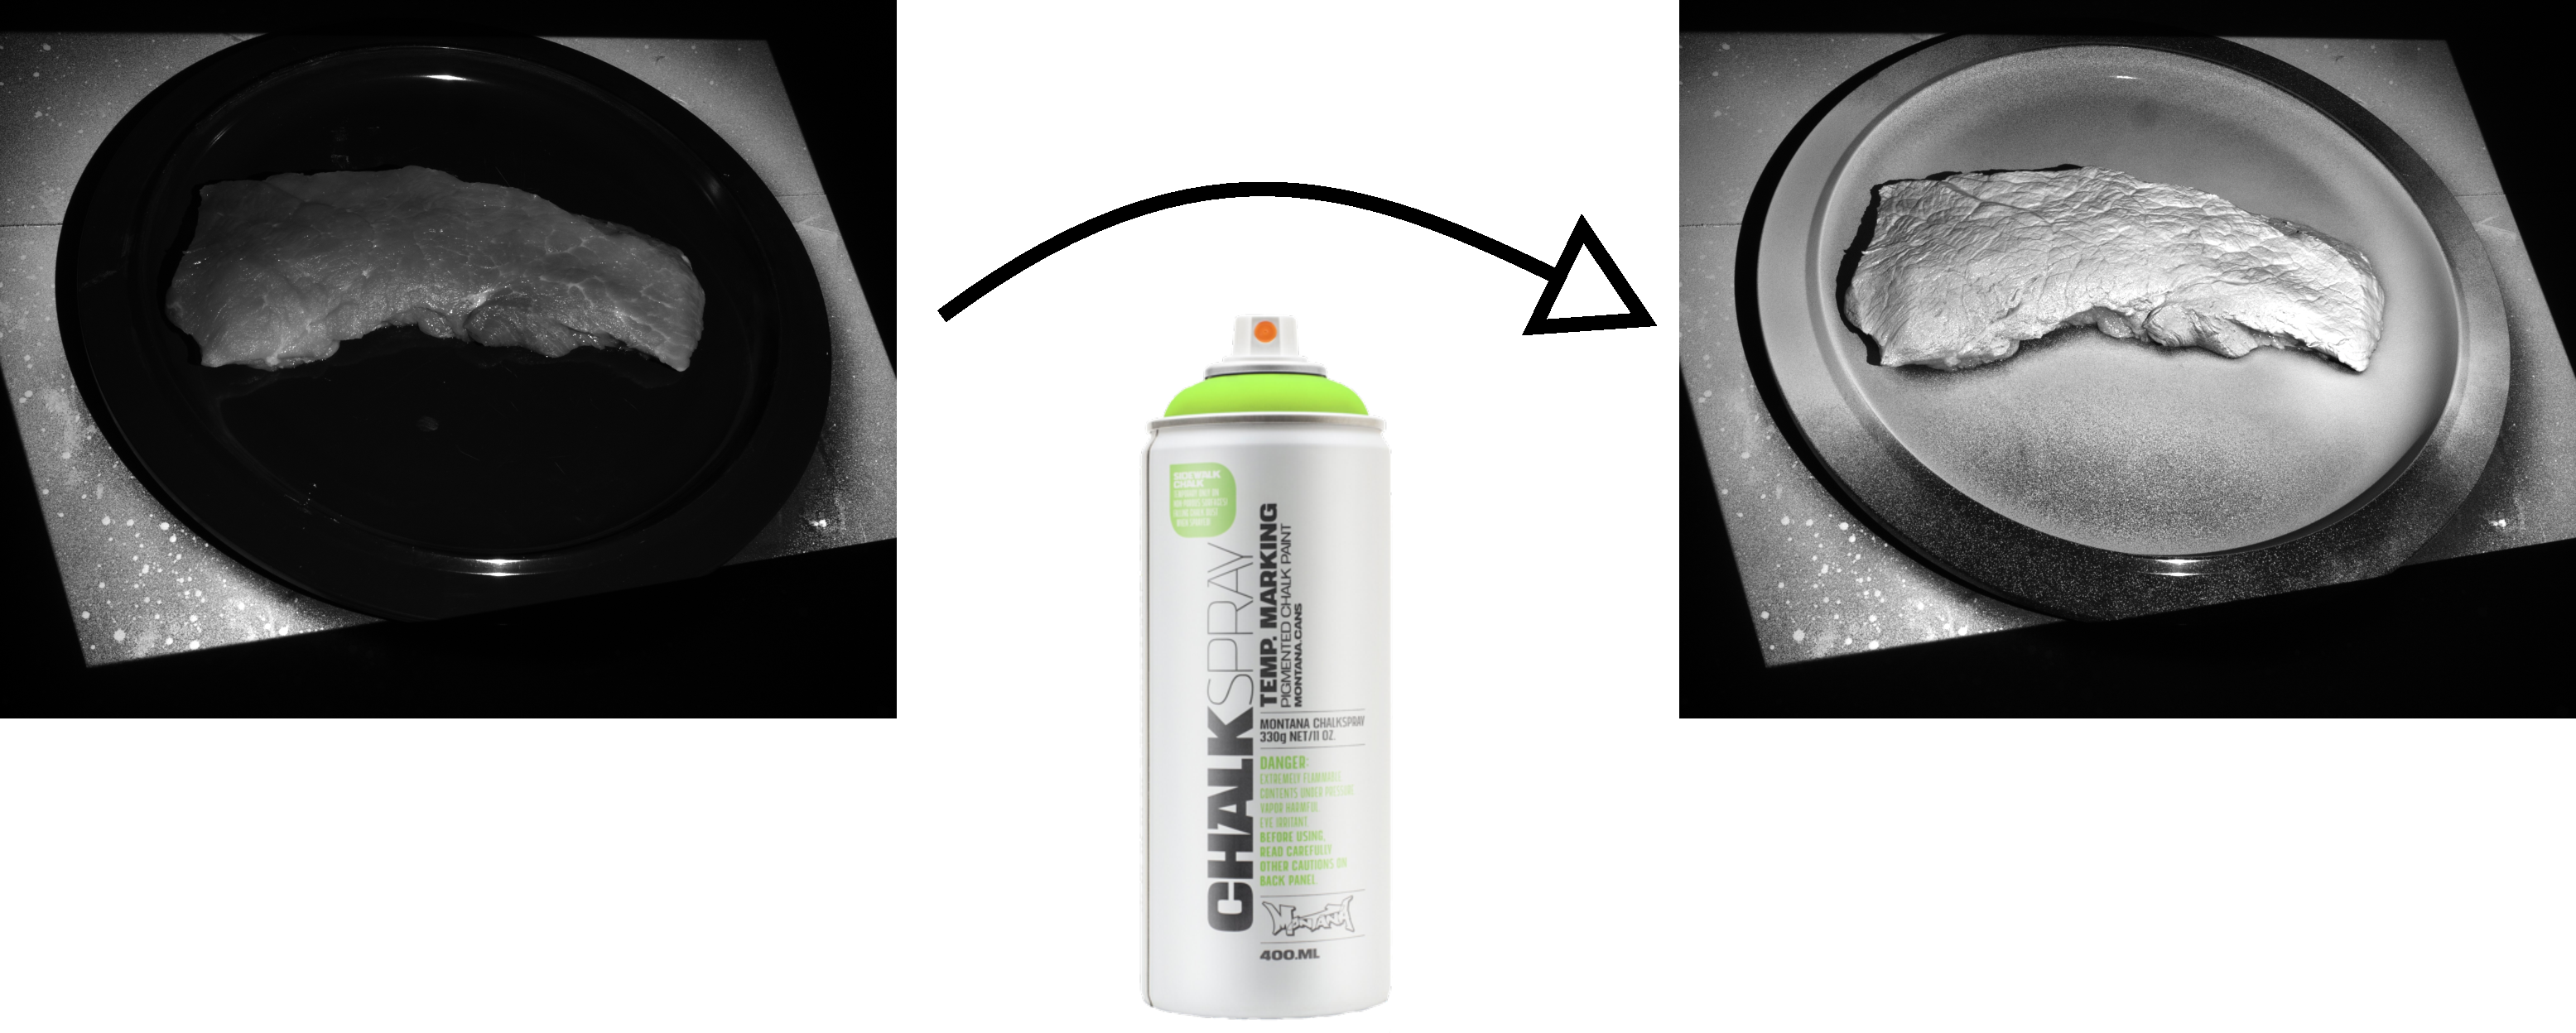
\includegraphics[width=0.95\linewidth]{figures/chalk_reference}
  \end{figure}
}

\frame{
  \frametitle{Boxplot of Reconstruction Error, Skin}
  \begin{figure}
    \centering
    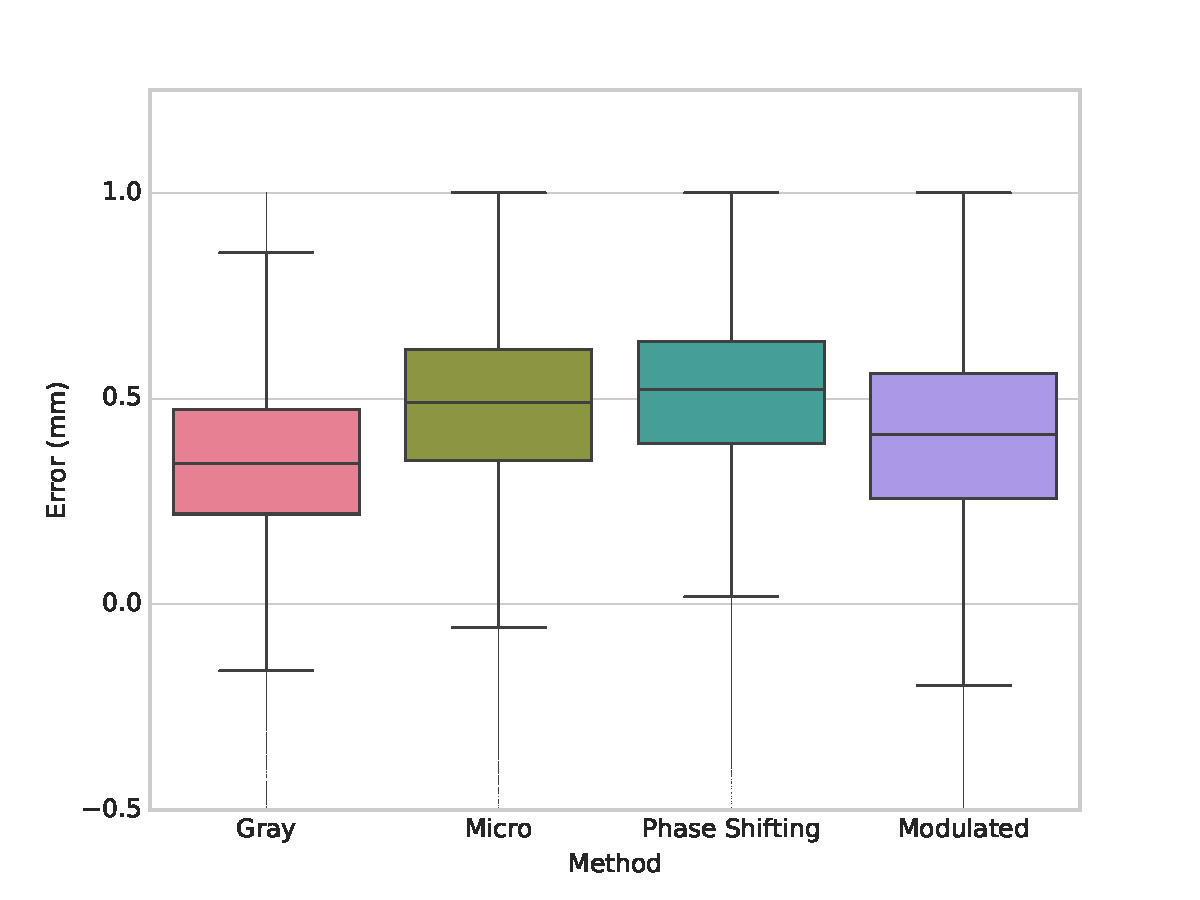
\includegraphics[height=0.85\textheight]{figures/boxplot_error}
  \end{figure}
}

\frame{
  \frametitle{Model}
  \begin{minipage}{0.48\textwidth}
    \begin{figure}
      \centering
      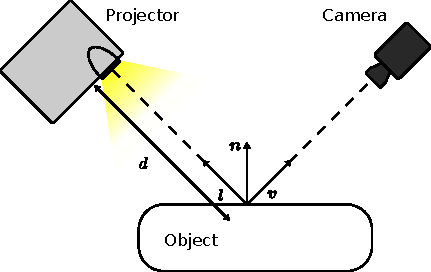
\includegraphics[height=0.65\textheight]{figures/camproj}
    \end{figure}
  \end{minipage}
  \hfill
  \begin{minipage}{0.48\textwidth}
    \begin{align}
      y = \begin{bmatrix} 1 & \mathbf{n} \cdot \mathbf{v} & \mathbf{n} \cdot \mathbf{l} & d \end{bmatrix}
      \begin{bmatrix}
        \beta_0\\
        \beta_1\\
        \beta_2\\
        \beta_3
      \end{bmatrix}
    \end{align}
  \end{minipage}
}

\frame{
\frametitle{Results}
  \begin{onlyenv}<1>
    \begin{table}
    \caption{Muscle model estimate and regression quality}
      \label{tab:parameters_muscle}
      %\centering

      \begin{tabular}{c|c c c c c c c c}
          & $\beta_0$ & $\beta_1$ & $\beta_2$ & $\beta_3$ & RMS$_\text{raw}$ & RMS$_\text{cor}$ & $R^2$ & $P$ \\\hline
          Gray & 0.13 & 0.15 & -0.026 & \num{2.3e-4} &  \textbf{0.42} & 0.27 & 0.0082 & 0 \\
          Phase Shifting & 0.25 & 0.47 & -0.18 & \num{-2.5e-5} & 0.5 & \textbf{0.21} & 0.06 & 0\\
          Micro PS & 0.21 & 0.36 & -0.12 & \num{-4.1e-6} & 0.45 & 0.23 & 0.034 & 0 \\
          Modulated PS & 0.27 & 0.077 & 0.053 & \num{-9.7e-5} & 0.42 & 0.26 & 0.0037 & 0
      \end{tabular}

      \vfill
      %\vspace{0.7cm}
      %\end{table}
      %\begin{table}[h]
      \caption{Skin model estimate and regression quality}
      \label{tab:parameters_skin}
        %\centering
      \begin{tabular}{c|c c c c c c c c}
          & $\beta_0$ & $\beta_1$ & $\beta_2$ & $\beta_3$ & RMS$_\text{raw}$ & RMS$_\text{cor}$ & $R^2$ & $P$ \\\hline
          Gray & -0.48 & 0.018 & 0.43 & \num{1.3e-3} &  \textbf{0.4} & 0.19 & 0.069 & 0 \\
          Phase Shifting & 0.27 &  0.28 & 0.26 & \num{-5.9e-4} &0.54 & \textbf{0.17} & 0.13 & 0\\
          Micro PS & 0.45 & 0.27 &  0.21 & \num{-1.0e-3} &  0.52 & 0.19 &  0.13 & 0 \\
          Modulated PS & 0.34 &  0.1 & 0.27 & \num{-6.7e-4} & 0.46 & 0.22 & 0.054 & 0
      \end{tabular}
    \end{table}
  \end{onlyenv}
  \begin{onlyenv}<2>
    \begin{table}
      %\vspace{0.7cm}
      %\end{table}
      %\begin{table}[h]
      \caption{Fat model estimate and regression quality}
      \label{tab:parameters_fat}
      \centering

      \begin{tabular}{c|c c c c c c c c}
          & $\beta_0$ & $\beta_1$ & $\beta_2$ & $\beta_3$ & RMS$_\text{raw}$ & RMS$_\text{cor}$ & $R^2$ & $P$ \\\hline
          Gray & -0.12 & 0.13 & 0.039 & \num{2.0e-4} & 0.26 & 0.24 & 0.016 & 0 \\
          Phase Shifting & -0.18 & 0.31 & -0.11 & \num{3.9e-4} & 0.22 & \textbf{0.16} & 0.084 & 0\\
          Micro PS & -0.13 &  0.2 & -0.043  &\num{3.0e-4} & \textbf{0.2} & 0.16 & 0.043 & 0\\
          Modulated PS & -0.06 & 0.15 & -0.029 & \num{1.6e-4}  &0.2  &0.17 & 0.018 & 0
      \end{tabular}
    \end{table}
  \end{onlyenv}
}

\frame{
  \frametitle{Conclusion}
  \begin{itemize}
    \item Subsurface scattering does not break structured light scanning.
    \item Reconstruction error is increased by up to 0.54mm RMS.
    \item Much of the error can be corrected with a general linear model.
  \end{itemize}
}

\section{Robotics \& Non-Rigid Objects}
\frame{
  \frametitle{An Adaptive Robotic System for Doing Pick and Place Operations with Deformable Objects}
  Troels Bo Jørgensen, Sebastian Nesgaard Jensen, Henrik Aanæs, Niels Worsøe Hansen and Nobert Krüger

  \textit{Robotics and Computer-Integrated Manufacturing (Under review, Accepted)}
  \begin{figure}
    \centering
    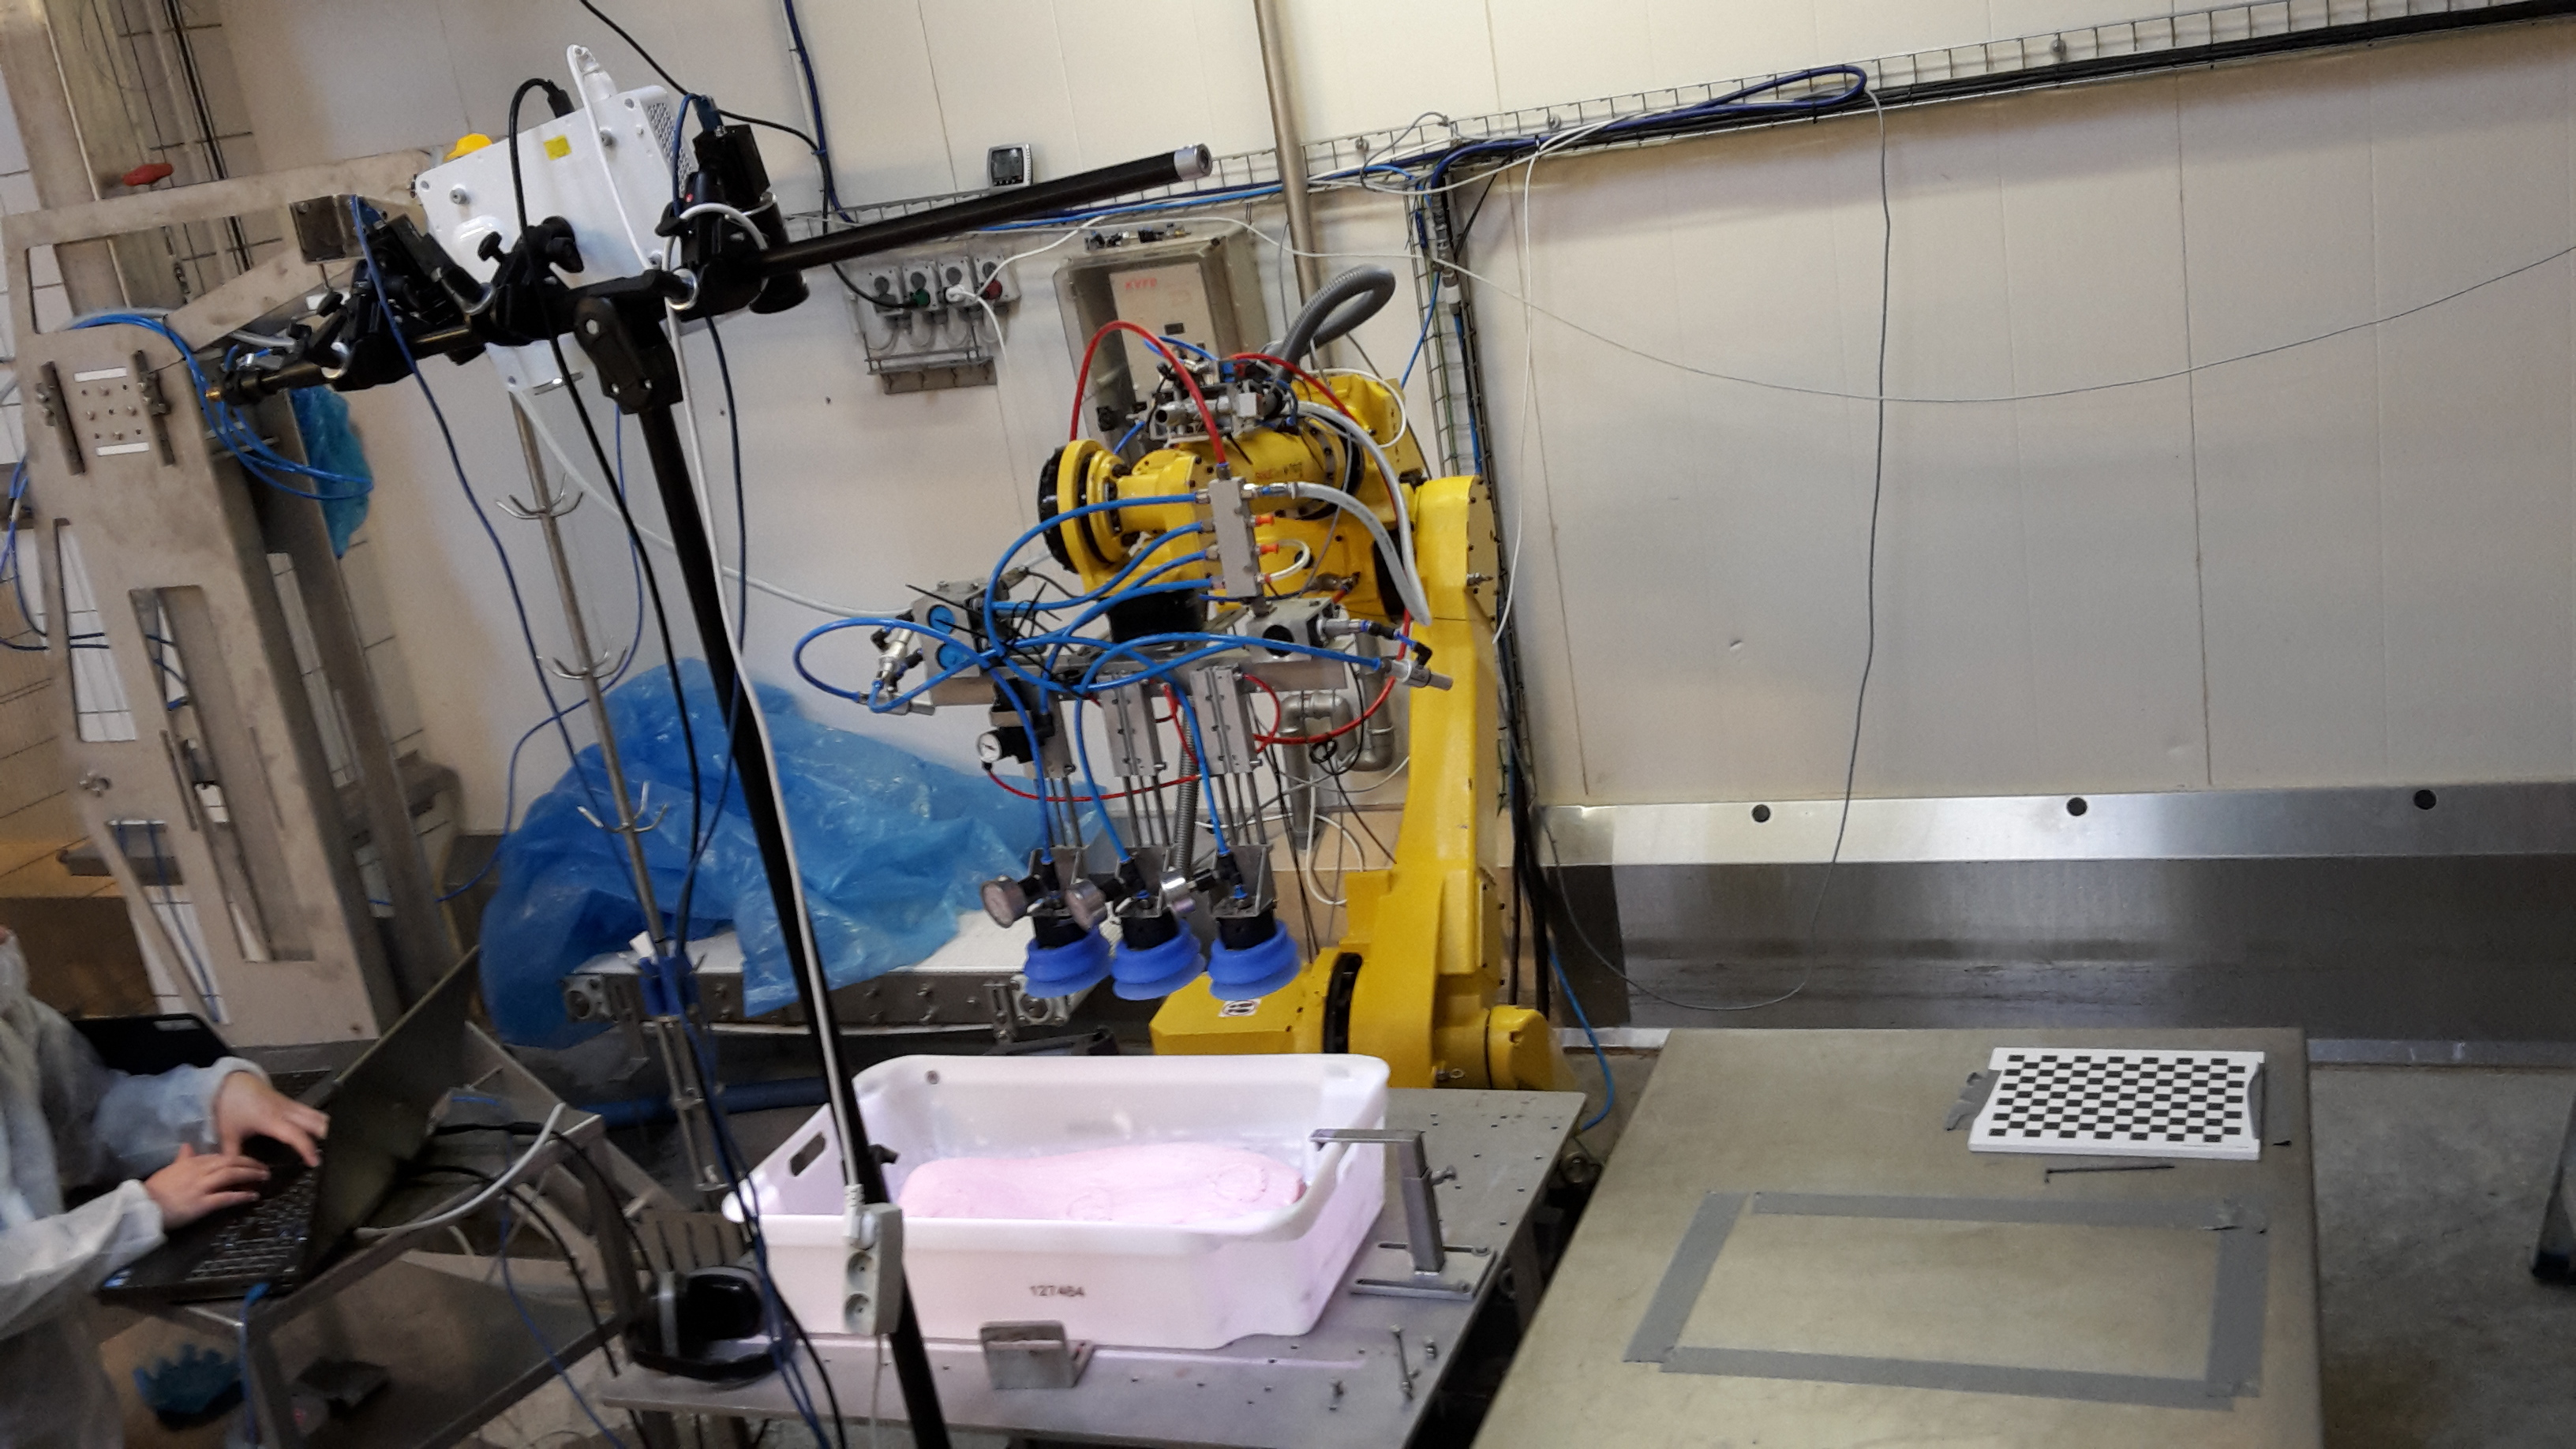
\includegraphics[height=0.65\textheight]{figures/dc_robot}
  \end{figure}
}

\frame{
  \frametitle{Guidance using Structured Light Scanning}
  \begin{figure}
    \centering
    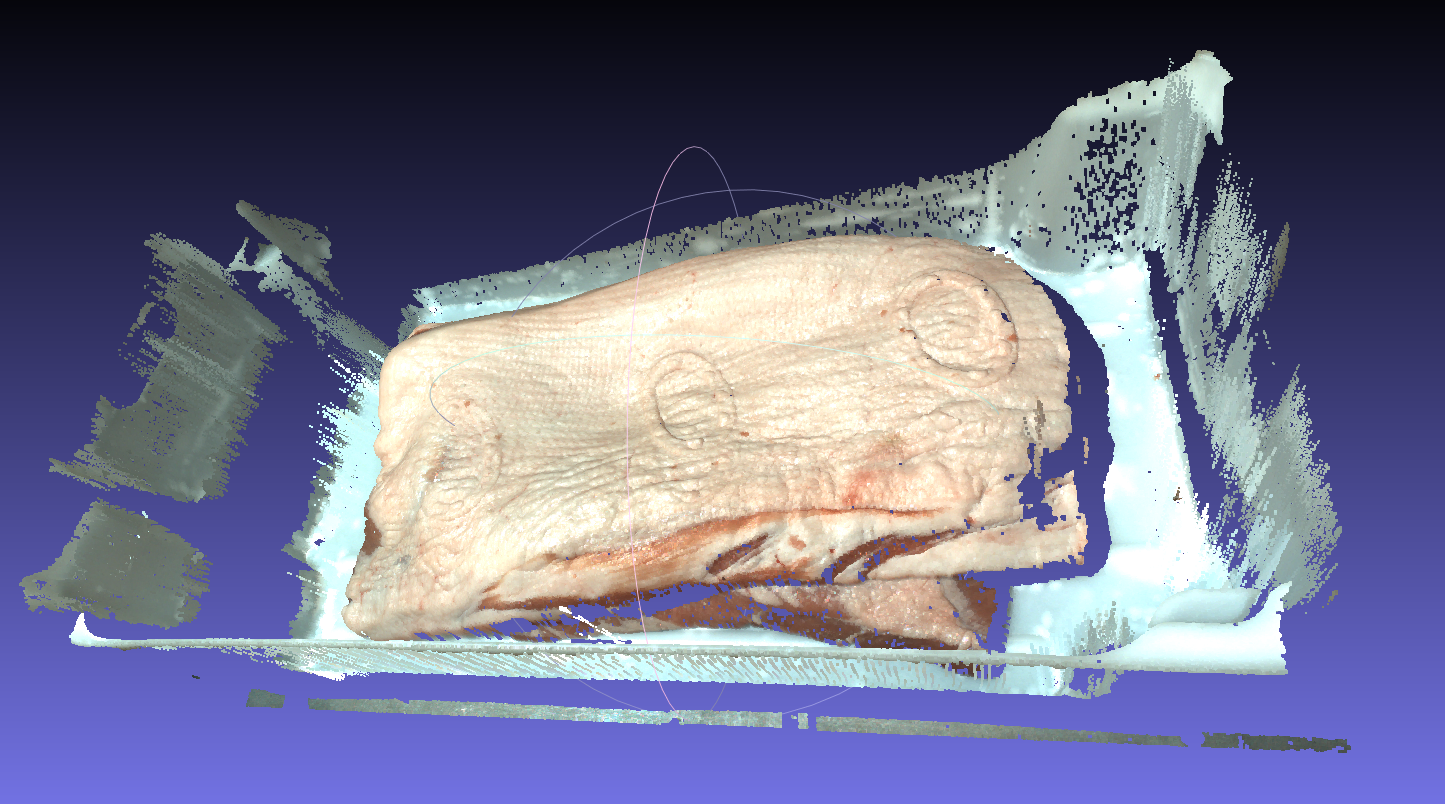
\includegraphics[height=0.6\textheight]{figures/dc_cloud}
    \hfill
    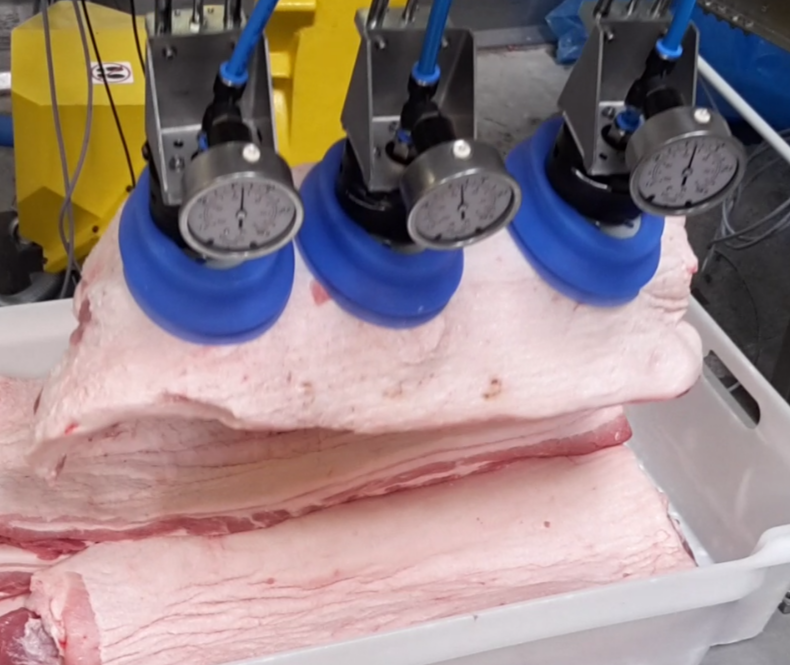
\includegraphics[height=0.6\textheight]{figures/dc_lift}
  \end{figure}
}

%\frame{
%  \frametitle{Segmentation}
%  \begin{figure}
%    \centering
%    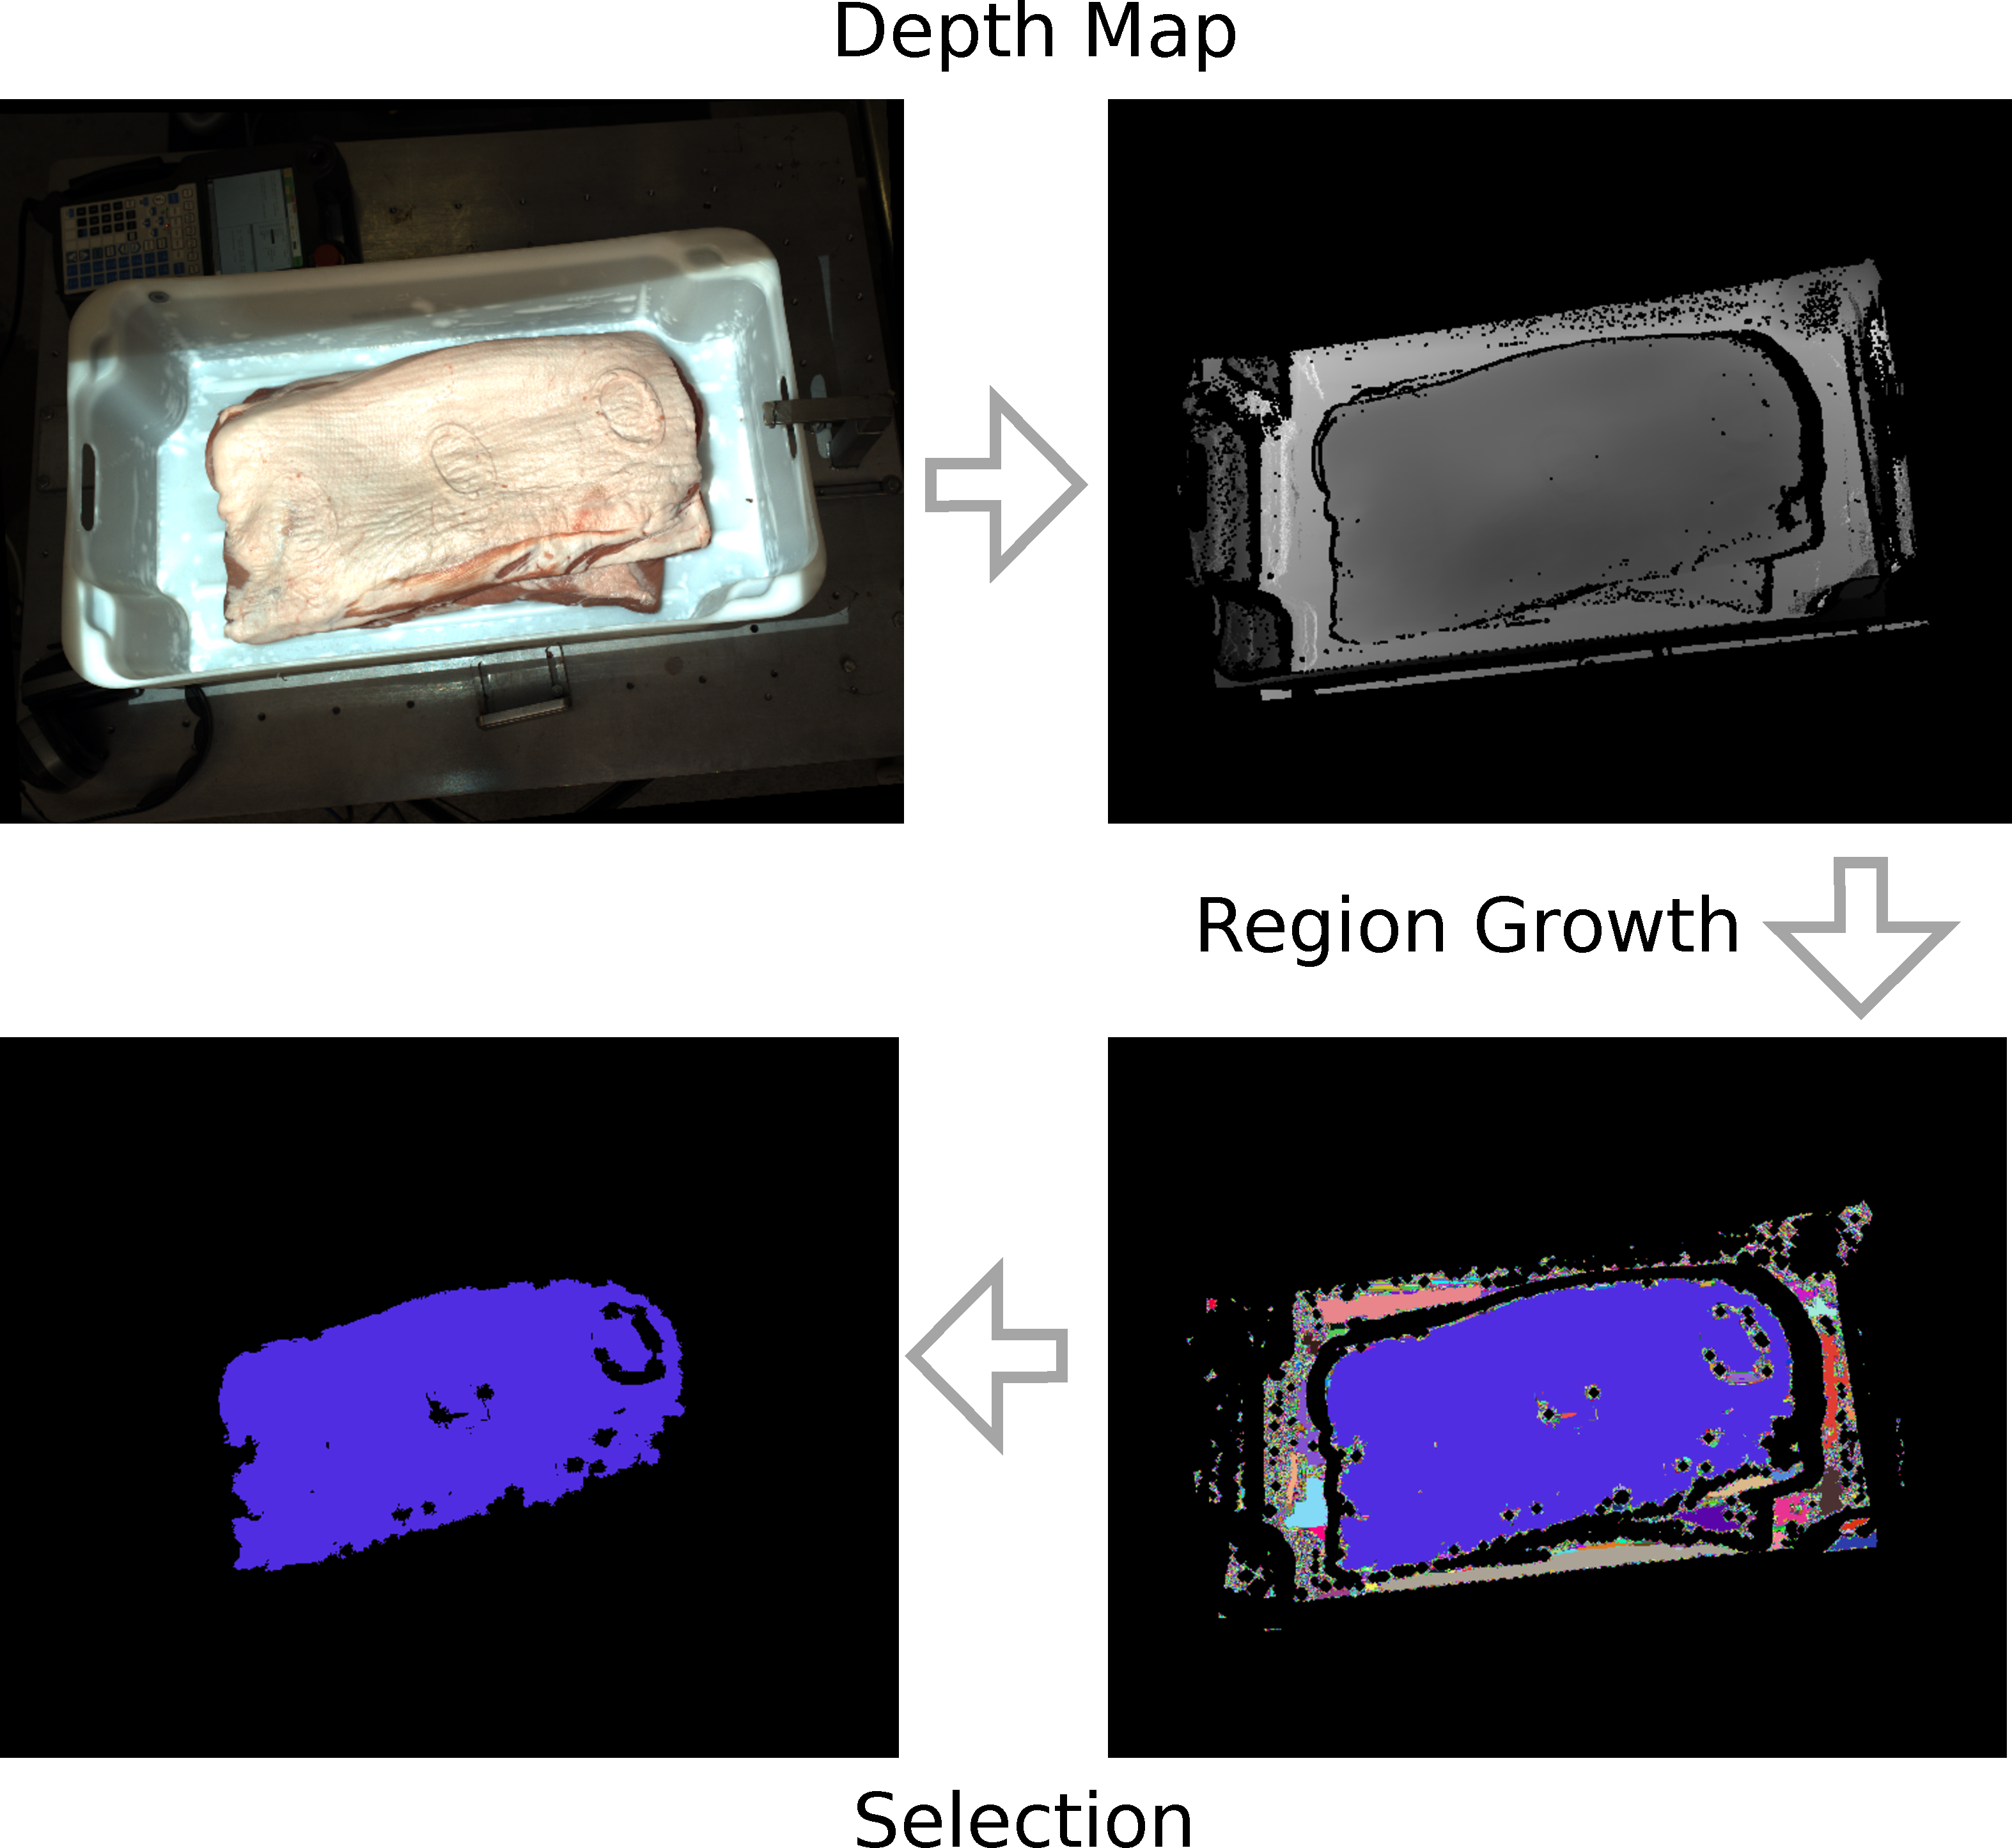
\includegraphics[height=0.9\textheight]{figures/dc_seg}
%  \end{figure}
%}

\frame{
  \frametitle{Demonstration}
  \begin{center}
    \movie[showcontrols, width = 1.35\textheight, height = 0.9\textheight, poster]{}{videos/succesDCManip.avi}
  \end{center}
}

\frame{
  \frametitle{Conclusion}
  \begin{itemize}
    \item Pick and place with deformable objects.
    \item Guidance using structured light.
    \item Working prototype demonstrated at Danish Crown, Ringsted.
  \end{itemize}
}

\section{Evaluation of NRSfM}
\frame{
  \frametitle{A Benchmark and Evaluation of Non-Rigid Structure from Motion}
  Sebastian Hoppe Nesgaard Jensen, Alessio Del Bue, Mads Emil Brix Doest and Henrik Aanæs

  \textit{IEEE Transactions on Pattern Analysis and Machine Intelligence (Under review)}
  \begin{figure}
    \centering
    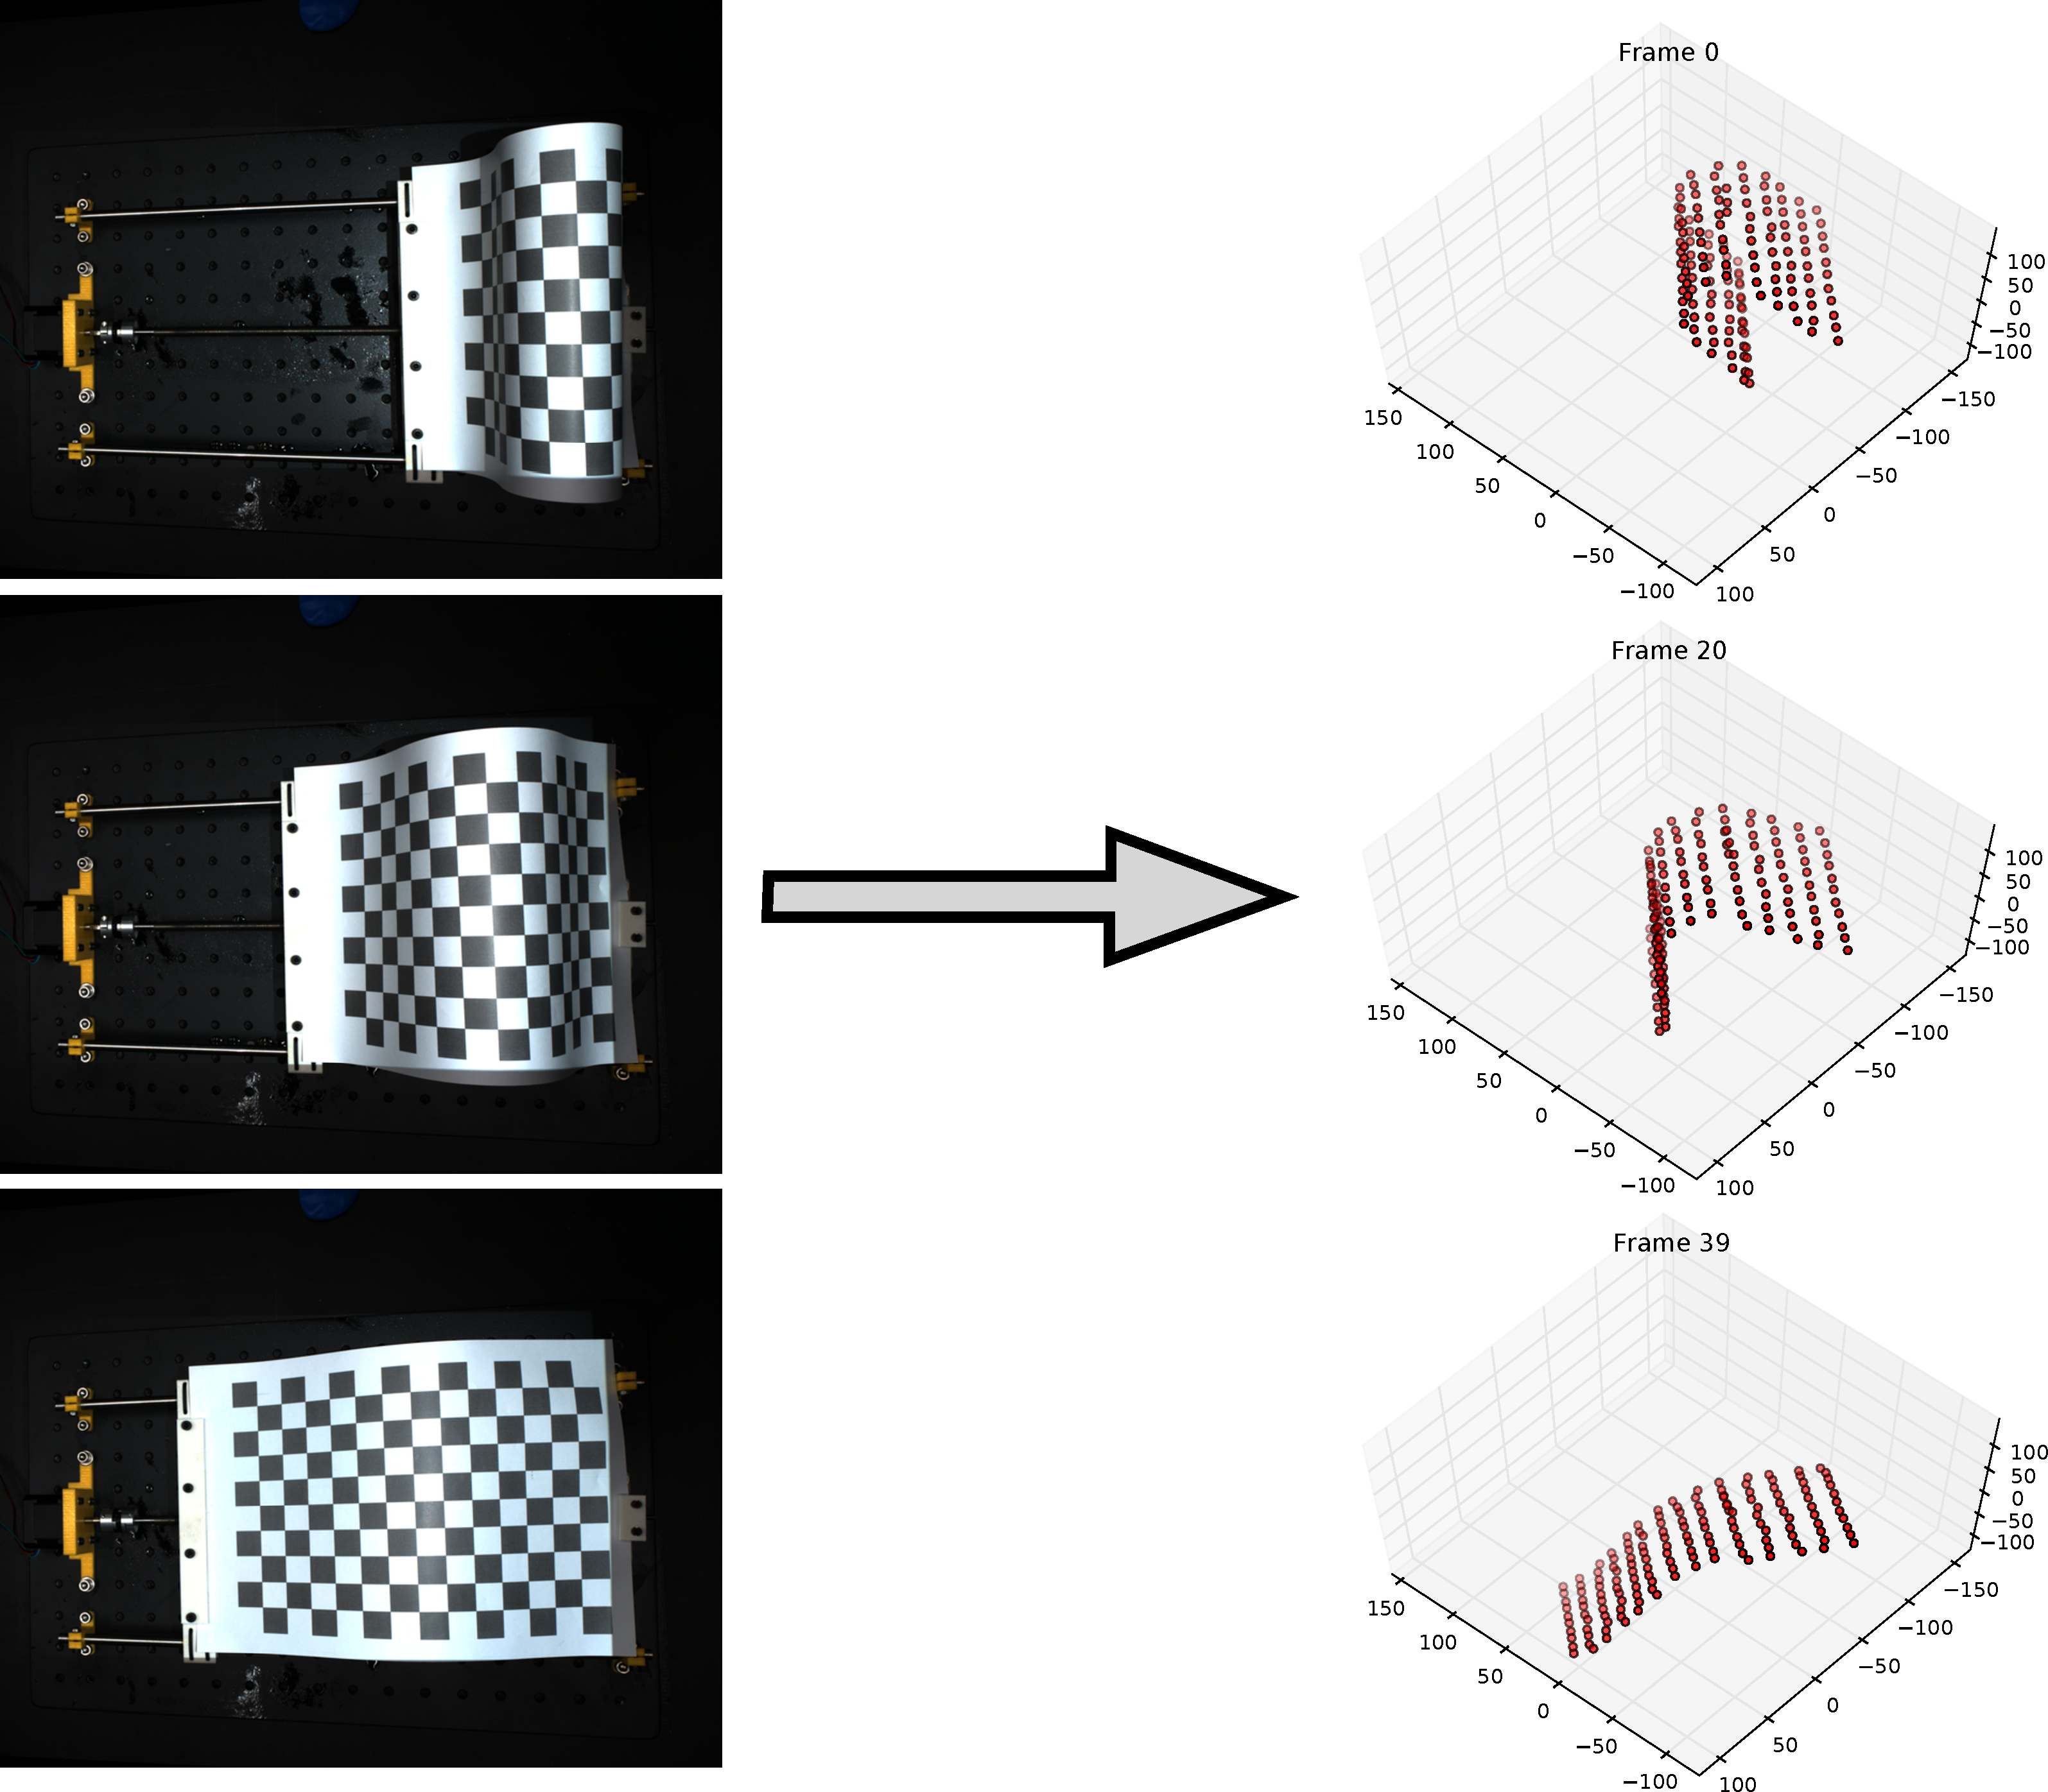
\includegraphics[height=0.65\textheight]{figures/nrsfm_paper_idea}
  \end{figure}
}

\begin{comment}
\frame{
  \frametitle{Structure-from-Motion}
  %\begin{figure}
  \begin{minipage}{0.48\textwidth}
    \begin{figure}
      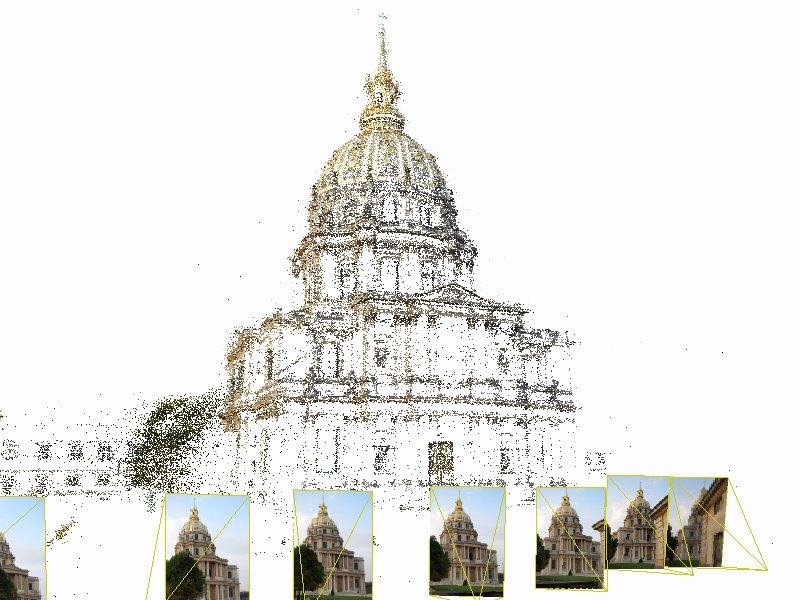
\includegraphics[height=0.65\textheight]{figures/sfm_0}
      \caption{\cite{enqvist2010stable}}
    \end{figure}
  \end{minipage}
  \hfill
  \begin{minipage}{0.48\textwidth}
    \begin{figure}
      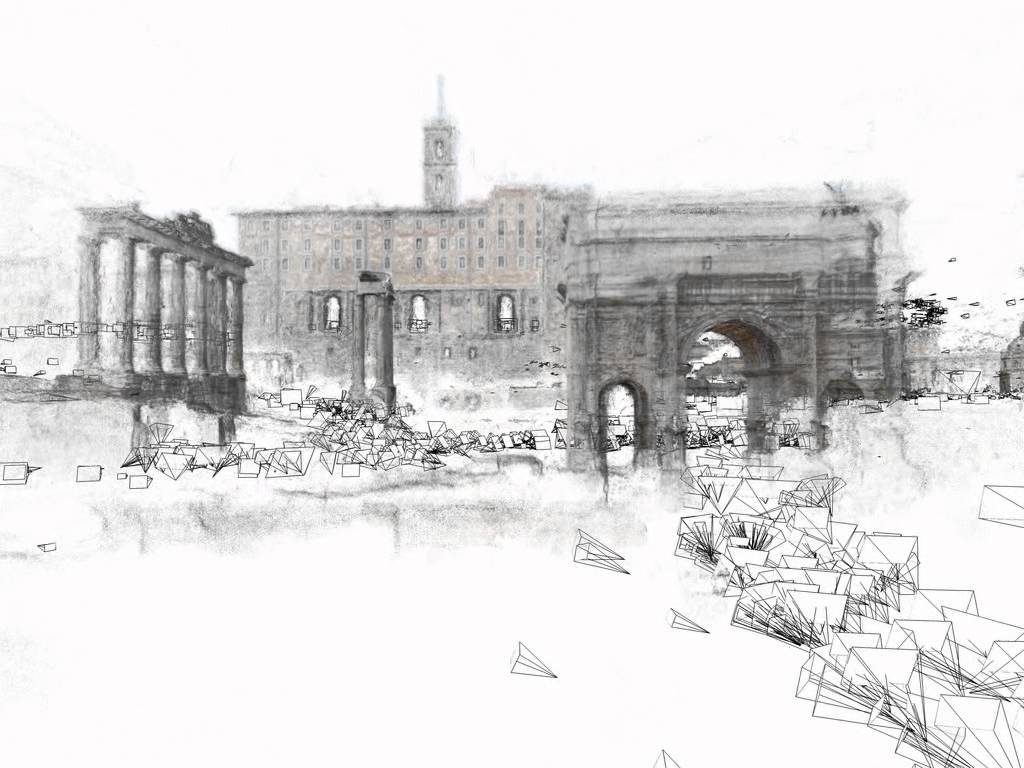
\includegraphics[height=0.65\textheight]{figures/sfm_1}
      \caption{\cite{crandall2011discrete}}
    \end{figure}
  \end{minipage}
  %\end{figure}
}
\end{comment}

\frame{
  \frametitle{Factorization of Structure-from-Motion}
  Assuming orthographic projection,
  \begin{align}
    \mathbf{W} = \mathbf{M}\mathbf{S}    \label{eq:nrsfm_fac}
  \end{align}
  \begin{align*}
    \mathbf{W} = \begin{bmatrix}
      \mathbf{w}_{11} & \mathbf{w}_{12} & \cdots & \mathbf{w}_{1P}\\
      \mathbf{w}_{21} & \mathbf{w}_{22} & \cdots & \mathbf{w}_{2P}\\
      \vdots   & \vdots   & \ddots & \vdots\\
      \mathbf{w}_{F1} & \mathbf{w}_{F2} & \cdots & \mathbf{w}_{FP}
    \end{bmatrix},
    \mathbf{M} = \begin{bmatrix}
      \mathbf{M}_1 & \mathbf{0}   & \cdots & \mathbf{0}\\
      \mathbf{0}   & \mathbf{M}_2 & \cdots & \mathbf{0}\\
      \vdots       & \vdots       & \ddots & \vdots    \\
      \mathbf{0}   & \mathbf{0}   & \cdots & \mathbf{M}_F
    \end{bmatrix},
    \mathbf{S} = \begin{bmatrix}
      \mathbf{s}_{11} & \mathbf{s}_{12} & \cdots & \mathbf{s}_{1P}\\
      \mathbf{s}_{21} & \mathbf{s}_{22} & \cdots & \mathbf{s}_{2P}\\
      \vdots       & \vdots       & \ddots & \vdots    \\
      \mathbf{s}_{F1} & \mathbf{s}_{F2} & \cdots & \mathbf{s}_{FP}
    \end{bmatrix}
  \end{align*}
}

\frame{
  \frametitle{Not Much Concensus on Priors}
  \begin{minipage}{0.48\textwidth}
    \begin{itemize}
      \item Low-rank basis
      \item DCT coefficients
      \item Spatial and temporal smoothness
      \item Clustering
      \item Perspective correction
      \item Compressibility
      \item And much more...
    \end{itemize}
  \end{minipage}
  \begin{minipage}{0.48\textwidth}
    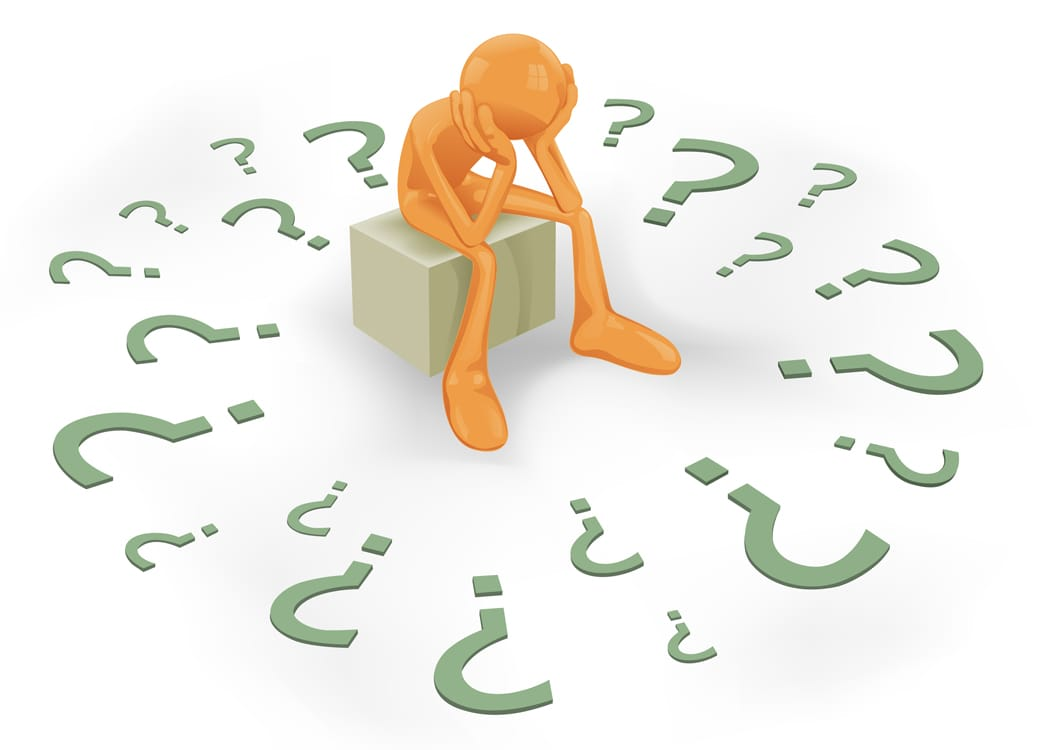
\includegraphics[width=\textwidth]{figures/confusion}
  \end{minipage}
}

\frame{
  \frametitle{Low-Rank Basis}
  \begin{align}
    \mathbf{s}_f = c_{f1}\mathbf{\hat{s}}_1 + c_{f2}\mathbf{\hat{s}}_2 + \cdots + c_{fK}\mathbf{\hat{s}}_K,\\
    \mathbf{W} = \underbrace{\mathbf{D}(\mathbf{C} \otimes \mathbf{I}_3)}_\mathbf{M}
    \underbrace{
      \begin{bmatrix}
        \mathbf{\hat{s}}_1\\
        \mathbf{\hat{s}}_2\\
        \vdots\\
        \mathbf{\hat{s}}_K
      \end{bmatrix}
    }_\mathbf{S},\label{eq:nrsfm_lowrank}
  \end{align}
  where,
  \begin{align*}
    \mathbf{D} = \begin{bmatrix}
      \mathbf{\hat{R}}_1 & \mathbf{0} & \cdots & \mathbf{0}\\
      \mathbf{0} & \mathbf{\hat{R}}_2 & \cdots & \mathbf{0}\\
      \vdots & \vdots & \ddots & \vdots\\
      \mathbf{0} & \mathbf{0}  & \cdots & \mathbf{\hat{R}}_F\\
    \end{bmatrix},
    \mathbf{C} &= \begin{bmatrix}
      c_{1, 1} & c_{1, 2} & \cdots & c_{1, K}\\
      c_{2, 1} & c_{2, 2} & \cdots & c_{2, K}\\
      \vdots & \vdots & \ddots & \vdots\\
      c_{F, 1} & c_{F, 2} & \cdots & c_{F, K}\\
    \end{bmatrix}
  \end{align*}
}

\frame{
  \frametitle{Temporal Smoothness using DCT}
  \begin{align}
    \mathbf{C} = \mathbf{\Omega}_T \begin{bmatrix}x_1& x_2 & \cdots & x_K\end{bmatrix} = \mathbf{\Omega}_T \mathbf{X},\\
    \mathbf{W} =  \underbrace{\mathbf{D}(\mathbf{\Omega}_T \mathbf{X} \otimes \mathbf{I}_3)}_\mathbf{M}
    \underbrace{
      \begin{bmatrix}
        \mathbf{\hat{s}}_1\\
        \mathbf{\hat{s}}_2\\
        \vdots\\
        \mathbf{\hat{s}}_K
      \end{bmatrix}
    }_\mathbf{S},
  \end{align}
  where,
  \begin{align*}
    \mathbf{\Omega}_T = \begin{bmatrix}
      \omega_{11} & \omega_{12} & \cdots & \omega_{1T}\\
      \omega_{21} & \omega_{22} & \cdots & \omega_{2T}\\
      \vdots      & \vdots      & \ddots & \vdots \\
      \omega_{F1} & \omega_{F2} & \cdots & \omega_{FT}\\
    \end{bmatrix},&
    \text{  }\omega_{ft} = \frac{\sigma_t}{\sqrt{F}}\cos{\frac{\pi (2f - 1)(t - 1)}{2F}},\\
    \sigma_t =& \begin{cases}
      1 & \text{if $t=1$}\\
      \sqrt{2} & \text{otherwise}
    \end{cases}
  \end{align*}
}

\frame{
  \frametitle{Missing Observations}
  \begin{minipage}{0.48\textwidth}
    The value of some $\mathbf{w}_{fp}$ are not known due to:
    \begin{itemize}
      \item Occlusions.
      \item Orientation relative to the camera.
    \end{itemize}
  \end{minipage}
  \begin{minipage}{0.48\textwidth}
    \begin{align}
      \mathbf{W} = \begin{bmatrix}
        \mathbf{w}_{11} & \xcancel{\mathbf{w}_{12}} & \cdots & \mathbf{w}_{1P}\\
        \mathbf{w}_{21} & \mathbf{w}_{22} & \cdots & \xcancel{\mathbf{w}_{2P}}\\
        \vdots   & \vdots   & \ddots & \vdots\\
        \mathbf{w}_{F1} & \xcancel{\mathbf{w}_{F2}} & \cdots & \mathbf{w}_{FP}
      \end{bmatrix}
    \end{align}
  \end{minipage}
}

\frame{
  \frametitle{Matrix Completion}
  \begin{algorithm}[H]
    \For{$k\in K$} {
      Fill missing entries: $\mathbf{Y}^{[k]} = Y(\mathbf{W}, \mathbf{Z}^{[k]})$\\
      Estimate centroid: $\mathbf{t}^{[k]} = \begin{bmatrix}
        E\left[\mathbf{y}^{[k]}_{1*}\right] & E\left[\mathbf{y}^{[k]}_{2*}\right] & \cdots & E\left[\mathbf{y}^{[k]}_{F*}\right]
      \end{bmatrix}^\mathrm{T}$\\
      Remove centroid: $\mathbf{\hat{Y}}^{[k]} = \mathbf{Y}^{[k]} - \begin{bmatrix} \mathbf{t}^{[k]} & \mathbf{t}^{[k]} & \cdots & \mathbf{t}^{[k]}  \end{bmatrix}$\\
      Solve NRSfM factorization: $\mathbf{\hat{Y}}^{[k]} = \mathbf{M}^{[k]}\mathbf{S}^{[k]}$\\
      Add centroid: $\mathbf{Z}^{[k + 1]} = \mathbf{M}^{[k]}\mathbf{S}^{[k]} + \begin{bmatrix} \mathbf{t}^{[k]} & \mathbf{t}^{[k]} & \cdots & \mathbf{t}^{[k]}  \end{bmatrix}$
    }
  \end{algorithm}
  As established by~\cite{paladini2009factorization}.
}

\frame{
  \frametitle{Previous Datasets}
  \setlength{\nrsfmwidth}{0.48\textwidth}
  \setlength{\nrsfmheight}{0.75\nrsfmwidth}
  \begin{center}
    %\movie[autostart, loop, width = 0.48\textwidth, height = 0.8\textheight, poster]{}{videos/shark.avi}
    \href{run:videos/shark.avi?autostart&loop}{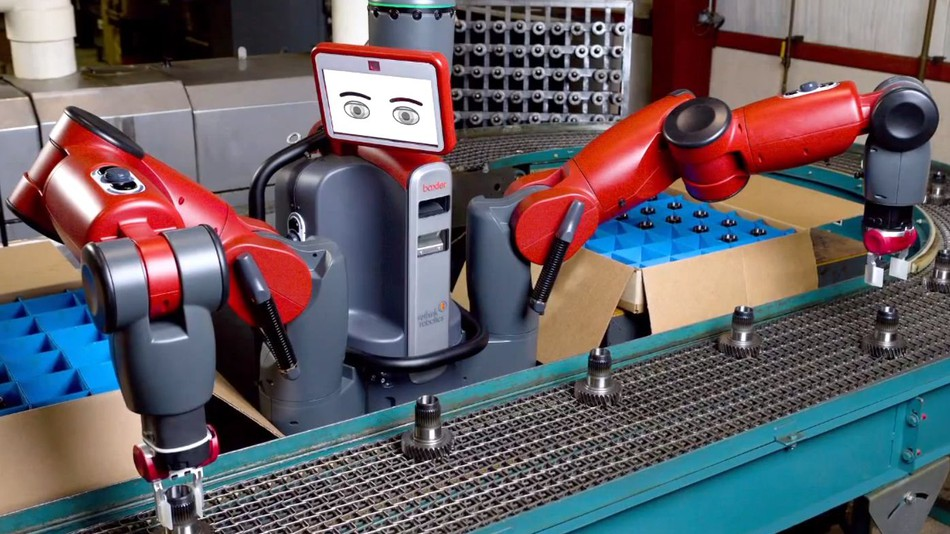
\includegraphics[width=\nrsfmwidth, height=\nrsfmheight]{figures/baxter.jpg}}
    \hfill
    %\movie[autostart, loop, width = 0.48\textwidth, height = 0.8\textheight, poster]{}{videos/walk.avi}
    \href{run:videos/walk.avi?autostart&loop}{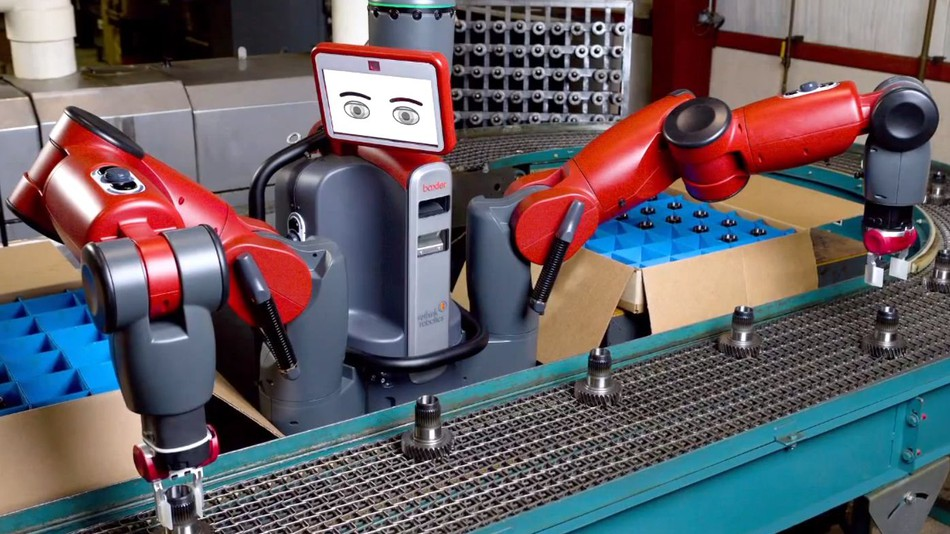
\includegraphics[width=\nrsfmwidth, height=\nrsfmheight]{figures/baxter.jpg}}
  \end{center}
  Animations and motion capture.
}

\frame{
  \frametitle{Important Questions}
  \begin{itemize}
    \item Which algorithms gives the best results on average?
    %\item Which types motions are the most difficult to reconstruct?
    \item How are missing observations best dealt with?
    \item How important is the assumption of an orthographic camera?
  \end{itemize}
}

\frame{
  \frametitle{Inspiration: Stop-Motion}
  \setlength{\nrsfmwidth}{0.48\textwidth}
  \setlength{\nrsfmheight}{0.6\nrsfmwidth}
  %\movie[autostart, loop, width = 0.48\textwidth, height = 0.7\textheight, poster]{}{videos/skeleton.avi}
  \href{run:videos/skeleton.avi?autostart&loop}{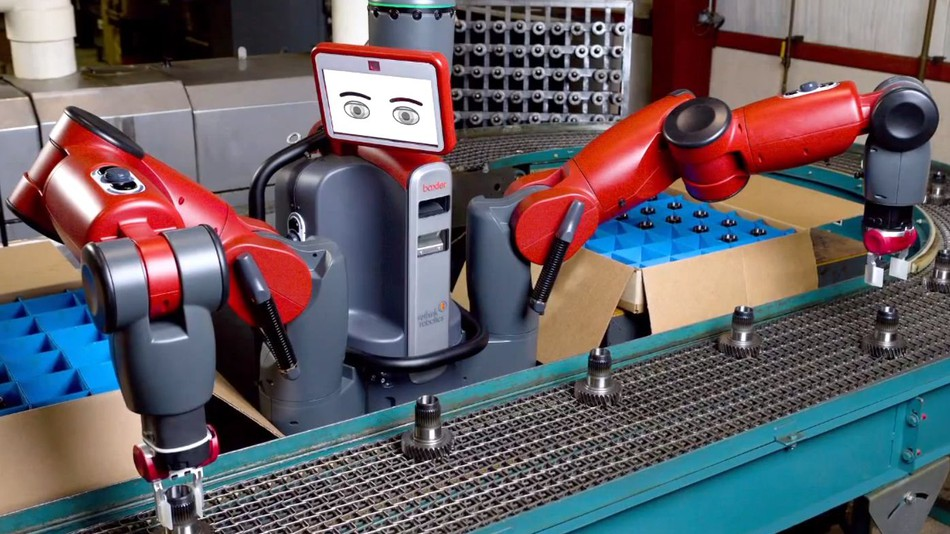
\includegraphics[width=\nrsfmwidth, height=\nrsfmheight]{figures/baxter.jpg}}
  \hfill
  \setlength{\nrsfmwidth}{0.48\textwidth}
  \setlength{\nrsfmheight}{0.688\nrsfmwidth}
  %\movie[autostart, loop, width = 0.48\textwidth, height = 0.7\textheight, poster]{}{videos/wallace.avi}
  \href{run:videos/wallace.avi?autostart&loop}{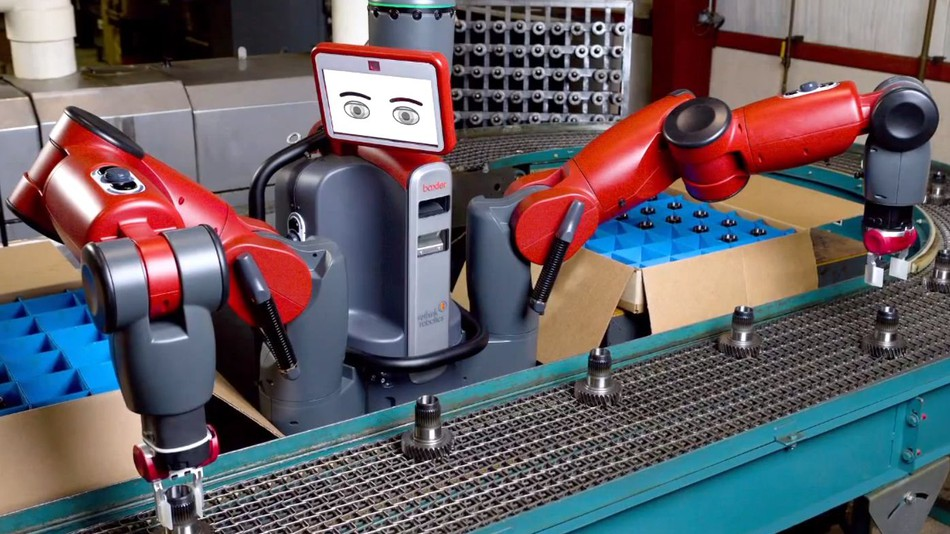
\includegraphics[width=\nrsfmwidth, height=\nrsfmheight]{figures/baxter.jpg}}
}

\frame{
  \setlength{\nrsfmwidth}{0.32\textwidth}
  \setlength{\nrsfmheight}{0.8009\nrsfmwidth}
  \href{run:videos/articulated/output.avi?autostart&loop}{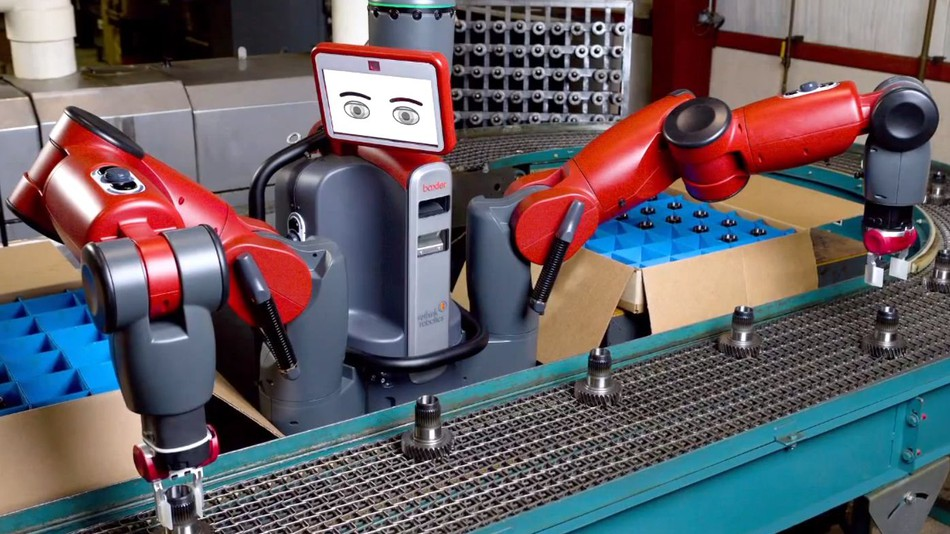
\includegraphics[width=\nrsfmwidth, height=\nrsfmheight]{figures/baxter.jpg}}
  %\movie[autostart, loop, width = 0.32\textwidth, height = 0.48\textheight]{}{videos/articulated/output.avi}
  \href{run:videos/balloon/output.avi?autostart&loop}{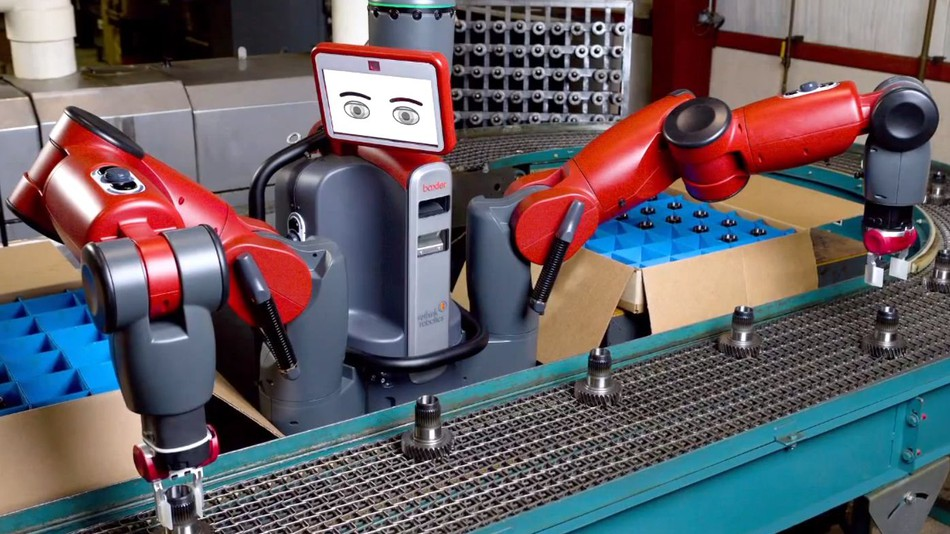
\includegraphics[width=\nrsfmwidth, height=\nrsfmheight]{figures/baxter.jpg}}
  %\movie[autostart, loop, width = 0.32\textwidth, height = 0.48\textheight]{}{videos/balloon/output.avi}
  \href{run:videos/paper/output.avi?autostart&loop}{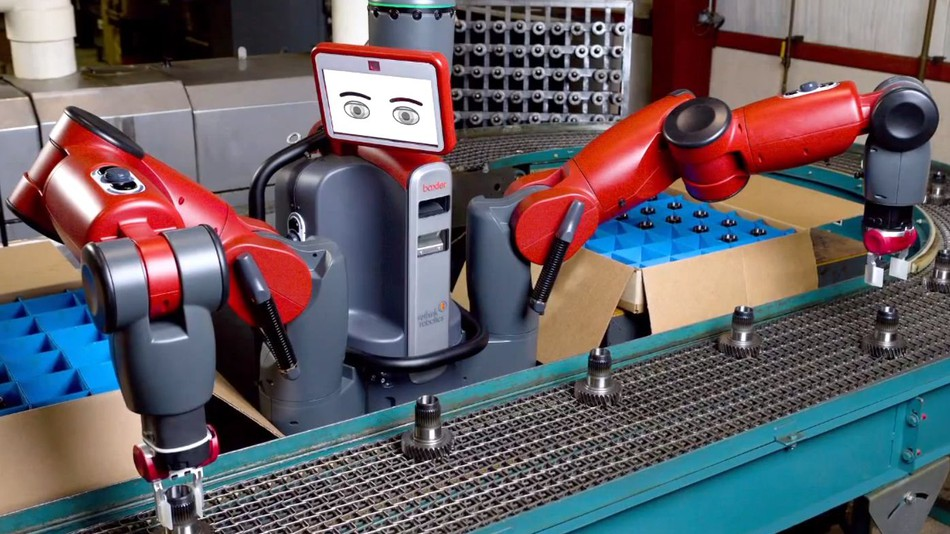
\includegraphics[width=\nrsfmwidth, height=\nrsfmheight]{figures/baxter.jpg}}
  %\movie[autostart, loop, width = 0.32\textwidth, height = 0.48\textheight]{}{videos/paper/output.avi}
  %\movie[autostart, loop, width = 0.32\textwidth, height = 0.48\textheight]{}{videos/paper.avi}
  %\movie[autostart, loop, width = 0.32\textwidth, height = 0.48\textheight]{}{videos/balloon.avi}
  \begin{center}
    \href{run:videos/stretch/output.avi?autostart&loop}{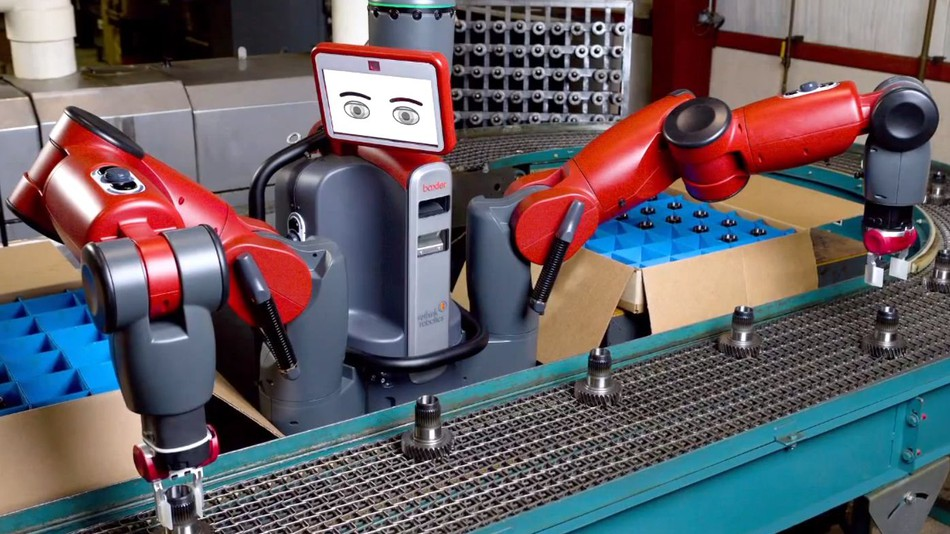
\includegraphics[width=\nrsfmwidth, height=\nrsfmheight]{figures/baxter.jpg}}
    %\movie[autostart, loop, width = 0.32\textwidth, height = 0.48\textheight]{}{videos/stretch/output.avi}
    \href{run:videos/tear/output.avi?autostart&loop}{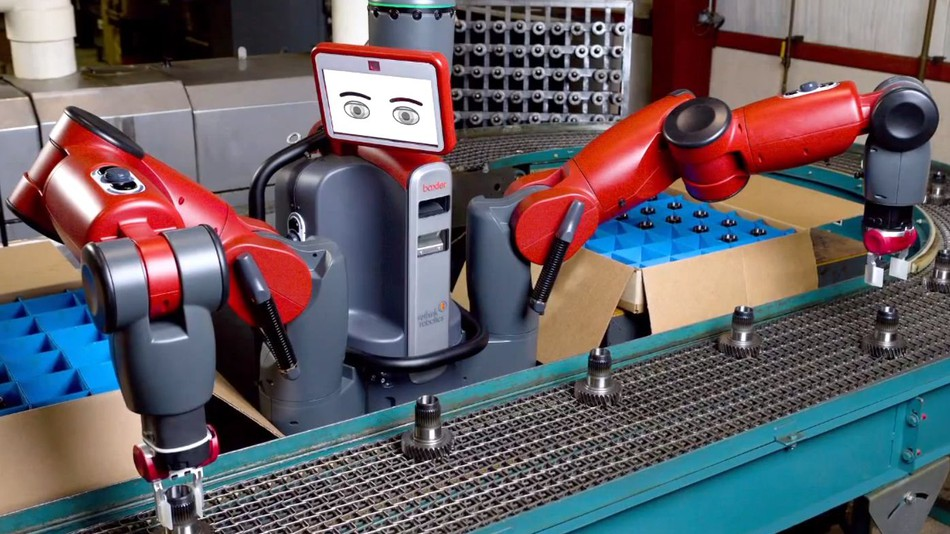
\includegraphics[width=\nrsfmwidth, height=\nrsfmheight]{figures/baxter.jpg}}
    %\movie[autostart, loop, width = 0.32\textwidth, height = 0.48\textheight]{}{videos/tear/output.avi}
  \end{center}
}

\frame{
  \frametitle{Recording Setup}
  \includegraphics[height = 0.7\textheight]{figures/nrsfm_cell}
  \hfill
  \includegraphics[height = 0.7\textheight]{figures/nrsfm_scanner}
}

\frame{
  \frametitle{Virtual Camera Paths}
  \begin{center}
    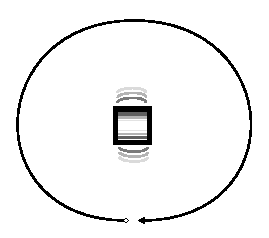
\includegraphics[height = 0.45\textheight]{figures/circle}
    \hfill
    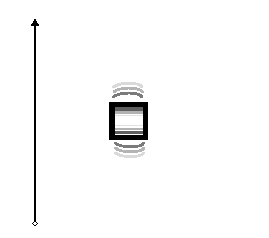
\includegraphics[height = 0.45\textheight]{figures/line}
    \hfill
    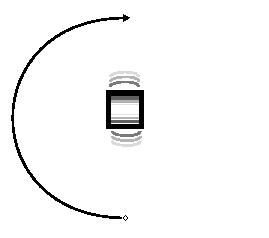
\includegraphics[height = 0.45\textheight]{figures/half_circle}
  \end{center}
  \begin{center}
    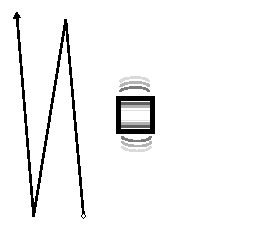
\includegraphics[height = 0.45\textheight]{figures/zigzag}
    \hfill
    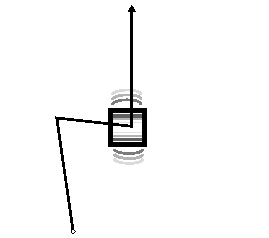
\includegraphics[height = 0.45\textheight]{figures/flyby}
    \hfill
    \includegraphics[height = 0.45\textheight]{figures/tricky}
  \end{center}
}

\frame{
  \frametitle{Observations}
  \setlength{\nrsfmwidth}{0.32\textwidth}
  \setlength{\nrsfmheight}{0.75\nrsfmwidth}
  \begin{center}
    \href{run:videos/observations/circle/output.avi?autostart&loop}{\includegraphics[width=\nrsfmwidth, height=\nrsfmheight]{figures/baxter.jpg}}
    %\movie[autostart, loop, width = 0.32\textwidth, height = 0.48\textheight]{}{videos/observations/circle/output.avi}
    \hfill
    \href{run:videos/observations/line/output.avi?autostart&loop}{\includegraphics[width=\nrsfmwidth, height=\nrsfmheight]{figures/baxter.jpg}}
    %\movie[autostart, loop, width = 0.32\textwidth, height = 0.48\textheight]{}{videos/observations/line/output.avi}
    \hfill
    \href{run:videos/observations/semi/output.avi?autostart&loop}{\includegraphics[width=\nrsfmwidth, height=\nrsfmheight]{figures/baxter.jpg}}
    %\movie[autostart, loop, width = 0.32\textwidth, height = 0.48\textheight]{}{videos/observations/semi/output.avi}
  \end{center}
  \begin{center}
    \href{run:videos/observations/zigzag/output.avi?autostart&loop}{\includegraphics[width=\nrsfmwidth, height=\nrsfmheight]{figures/baxter.jpg}}
    %\movie[autostart, loop, width = 0.32\textwidth, height = 0.48\textheight]{}{videos/observations/zigzag/output.avi}
    \hfill
    \href{run:videos/observations/flyby/output.avi?autostart&loop}{\includegraphics[width=\nrsfmwidth, height=\nrsfmheight]{figures/baxter.jpg}}
    %\movie[autostart, loop, width = 0.32\textwidth, height = 0.48\textheight]{}{videos/observations/flyby/output.avi}
    \hfill
    \href{run:videos/observations/tricky/output.avi?autostart&loop}{\includegraphics[width=\nrsfmwidth, height=\nrsfmheight]{figures/baxter.jpg}}
    %\movie[autostart, loop, width = 0.32\textwidth, height = 0.48\textheight]{}{videos/observations/tricky/output.avi}
  \end{center}
}

\frame{
  \frametitle{Missing Observations}
  \setlength{\nrsfmwidth}{0.32\textwidth}
  \setlength{\nrsfmheight}{0.75\nrsfmwidth}
  \begin{center}
    \href{run:videos/missingdata/circle/output.avi?autostart&loop}{\includegraphics[width=\nrsfmwidth, height=\nrsfmheight]{figures/baxter.jpg}}
    %\movie[autostart, loop, width = 0.32\textwidth, height = 0.48\textheight]{}{videos/missingdata/circle/output.avi}
    \hfill
    \href{run:videos/missingdata/line/output.avi?autostart&loop}{\includegraphics[width=\nrsfmwidth, height=\nrsfmheight]{figures/baxter.jpg}}
    %\movie[autostart, loop, width = 0.32\textwidth, height = 0.48\textheight]{}{videos/missingdata/line/output.avi}
    \hfill
    \href{run:videos/missingdata/semi/output.avi?autostart&loop}{\includegraphics[width=\nrsfmwidth, height=\nrsfmheight]{figures/baxter.jpg}}
    %\movie[autostart, loop, width = 0.32\textwidth, height = 0.48\textheight]{}{videos/missingdata/semi/output.avi}
  \end{center}
  \begin{center}
    \href{run:videos/missingdata/zigzag/output.avi?autostart&loop}{\includegraphics[width=\nrsfmwidth, height=\nrsfmheight]{figures/baxter.jpg}}
    %\movie[autostart, loop, width = 0.32\textwidth, height = 0.48\textheight]{}{videos/missingdata/zigzag/output.avi}
    \hfill
    \href{run:videos/missingdata/flyby/output.avi?autostart&loop}{\includegraphics[width=\nrsfmwidth, height=\nrsfmheight]{figures/baxter.jpg}}
    %\movie[autostart, loop, width = 0.32\textwidth, height = 0.48\textheight]{}{videos/missingdata/flyby/output.avi}
    \hfill
    \href{run:videos/missingdata/tricky/output.avi?autostart&loop}{\includegraphics[width=\nrsfmwidth, height=\nrsfmheight]{figures/baxter.jpg}}
    %\movie[autostart, loop, width = 0.32\textwidth, height = 0.48\textheight]{}{videos/missingdata/tricky/output.avi}
  \end{center}
}

\frame{
  \frametitle{Algorithm Performance without Missing Observations}
  \begin{table}[!t]
  \centering
  %\caption{Averages given in milimeters.}
  %\label{table:full_linear_algo}

  \begin{tabular}{r r r r}\toprule
    \textbf{MultiBody} & \textbf{KSTA} & \textbf{RIKS} & \textbf{CSF2}\\
    29.36 & 31.94 & 32.21 & 32.83\\ \midrule
    \textbf{MetricProj} & \textbf{CSF} & \textbf{Bundle} & \textbf{PTA}\\
    34.09 & 41.19 & 46.66 & 46.80\\ \midrule
    \textbf{ScalableSurface} & \textbf{EM PPCA} & \textbf{SoftInext} & \textbf{BALM}\\
    53.88 & 59.19 & 61.94 & 66.34\\ \midrule
    \textbf{MDH} & \textbf{Compressible} & \textbf{SPFM} & \textbf{Consensus}\\
    70.34 & 79.18 & 85.34 & 94.61\\ \midrule
  \end{tabular}
\end{table}
Numbers are averages given in milimeters.
}

\frame{
  \frametitle{Error Distribution of the Top Five Algorithms}
  \begin{minipage}{0.45\textwidth}
    \begin{itemize}
      \item Equal mean performance.
      \item One-way ANOVA p-value of 0.18.
    \end{itemize}
  \end{minipage}
  \begin{minipage}{0.45\textwidth}
    \begin{center}
      \includegraphics[height = 0.8\textheight]{figures/boxplot_error_noncorrect}
    \end{center}
  \end{minipage}
  Adjusted for influence of other factors such as camera model, deformation type etc.
}

\frame{
  \frametitle{Influence of Missing Observations}
  \begin{minipage}{0.45\textwidth}
    \begin{itemize}
      \item Only MetricProj is relatively stable.
      \item BALM decrease in error is probably a fluke (due to bad performance).
      \item One-way ANOVA p-value of 0.018.
    \end{itemize}
  \end{minipage}
  \begin{minipage}{0.45\textwidth}
    \begin{figure}
      \includegraphics[height = 0.7\textheight]{figures/boxplot_error_noncorrect_mis}
    \end{figure}
  \end{minipage}
  \begin{center}
    \includegraphics[width = \textwidth]{figures/miss_algo}
  \end{center}
  %Numbers are averages given in milimeters.
}

\frame{
  \frametitle{Influence of the Camera Model}
  \begin{minipage}{0.45\textwidth}
    \begin{itemize}
      \item Each point represents the reconstruction error of a combination of algorithm, camera path and deformation with input created using either orthographic or perspective projection.
      \item fitted a line gives $y = 0.96x + 4.06$.
      \item ANOVA indicates a mean increase in error of $7.2$mm.
      \item State-of-the-art does not "break" under perspective projection.
      \item Bear limited spatial extend of data in mind.
    \end{itemize}
  \end{minipage}
  \begin{minipage}{0.45\textwidth}
    \begin{center}
      \includegraphics[height = 0.8\textheight]{figures/ort_per_scatter}
    \end{center}
  \end{minipage}
}

\frame{
  \frametitle{Conclusion}
  \begin{description}
    \item[Which algorithms gives the best results on average?] \hfill \\ Established ranking of NRSfM algorithms. Missing observation experiments points to MetricProj.
    \item[How are missing observations best dealt with?] \hfill\\ Many methods are unable to handle occlusion-based missing observations. MetricProj seems to be the only stable one.
    \item[How important is the assumption of an orthographic camera?] \hfill \\ Orthographic assumptions works under perspective projection, though with increased reconstruction error.
  \end{description}

  Consider implementing MetricProj matrix completion algorithm for filling missing observations.
}

\section{The End}

\begin{comment}
  \frame{
    \frametitle{Perspective}
    \begin{center}
      \includegraphics[height=0.8\textheight]{figures/horizon}
    \end{center}
  }

  \frame{
    \frametitle{Perspective}

  }
\end{comment}

\frame{
  \frametitle{The End}
  %\begin{itemize}
  %  \item 3D vision can be used solve real-world problems.
  %  \item Attention should be paid to non-rigid objects.
  %\end{itemize}
  Thank you very much!
}



\frame{
	\frametitle{References}
	\bibliographystyle{ieeetr}
	{\small \bibliography{biblio}}
}

\end{document}
